\documentclass[11pt]{article}

\usepackage[margin=1in]{geometry}
\usepackage[T1]{fontenc}   % proper glyphs + copyable/searchable PDF text
\usepackage{lmodern}
\usepackage{microtype}     % better justification, fewer overfull lines
\usepackage{amsmath}
\usepackage{amssymb}
\usepackage{graphicx}
\usepackage{array}
\usepackage{booktabs}
\usepackage{float}
\usepackage{seqsplit}
\usepackage{tikz}
\usetikzlibrary{arrows.meta,positioning,fit,calc,decorations.pathmorphing}
\usepackage{hyperref} % last, so it patches float correctly

\hypersetup{
  colorlinks=true,
  linkcolor=blue,
  urlcolor=blue,
  pdftitle={How the RREA Model Is Built on WarpX/AMReX: A Beginner-Friendly
    Architecture Guide},
  pdfauthor={RREA WarpX/AMReX project},
  pdfsubject={Architecture of the RREA / relativistic-feedback simulation
    model built on WarpX and AMReX},
  pdfkeywords={RREA, relativistic feedback, TGF, WarpX, AMReX,
    particle-in-cell, Monte Carlo transport}
}

\setlength{\parindent}{0pt}
\setlength{\parskip}{0.7em}
\renewcommand{\arraystretch}{1.18}
\emergencystretch=1.5em
% Let long code paths break at separators (used via \path{...}):
\def\UrlBreaks{\do\/\do\_\do\-\do\.\do\=\do\:}
\DeclareRobustCommand{\code}[1]{\texttt{\seqsplit{#1}}}

% The figures' shared colour grammar, defined ONCE: orange = RREA code,
% blue = stock WarpX, green = the native library/fluid family.  The darker
% edge colours are the grayscale channel -- orange!12 and blue!8 collapse to
% the same gray in print, the borders do not.
\colorlet{rreafill}{orange!12}
\colorlet{rreaedge}{orange!60!black}
\colorlet{warpxfill}{blue!8}
\colorlet{warpxedge}{blue!50!black}
\colorlet{nativefill}{green!10}

\title{How the RREA Model Is Built on WarpX/AMReX:\\
A Beginner-Friendly Architecture Guide}
\author{RREA WarpX/AMReX project}
\date{}

\begin{document}
\maketitle

\begin{abstract}
This guide explains, from first principles, how the RREA (Relativistic
Runaway Electron Avalanche) and \textbf{relativistic feedback} simulation
model is constructed on top of two open-source frameworks: \textbf{AMReX}
(a block-structured mesh and particle library) and \textbf{WarpX} (a
particle-in-cell plasma code built on AMReX). The model tracks not only the
forward electron avalanches but also the backward-propagating bremsstrahlung
photons and pair-produced positrons that can re-seed new avalanches at the
source region --- Dwyer's relativistic feedback mechanism, which turns
isolated avalanches into a self-sustaining discharge and is essential for
Terrestrial Gamma-ray Flash physics. The guide is written for a reader who
knows basic plasma/atmospheric physics and some C++, but who has never used
WarpX or AMReX. It describes what the frameworks provide out of the box,
exactly where and how the RREA code attaches to them, what happens during
one simulation time step, and why the project is organized the way it is.
It documents the schema-6 transport and Maxwell TM engine.
\end{abstract}

\tableofcontents
\newpage

\paragraph*{How to read this guide.} If you are new to the project, read
Sections~\ref{sec:physics}--\ref{sec:blocks} for the physics goal and a
five-minute tour of AMReX and WarpX, then
Sections~\ref{sec:overlay}--\ref{sec:deck} for how the code attaches to WarpX
and what the input deck controls. The heart of the guide is the walkthrough of one
simulation time step (Section~\ref{sec:step}); nearly every later section
expands one box of its data-flow figure. The deeper dives --- the
interaction tables (Section~\ref{sec:tables}), the avalanche-length
benchmark (Section~\ref{sec:cdcheck}), and the fluid and field solve
(Section~\ref{sec:field}) --- can be read independently, as can the
diagnostics and observable-signature sections. Recurring terms are
collected in the Glossary at the end.

%=====================================================================
\section{What the Model Simulates}\label{sec:physics}

A thundercloud can sustain quasi-static electric fields above the
\emph{runaway breakeven} threshold. In such fields, an energetic electron
(MeV scale) gains more energy from the field than it loses to air, so it
``runs away,'' and its hard collisions knock out further energetic
electrons: a Relativistic Runaway Electron Avalanche. The avalanche emits
bremsstrahlung gamma rays (the mechanism behind Terrestrial Gamma-ray
Flashes), creates positrons, and --- crucially --- also deposits an enormous
number of \emph{low-energy} electrons and ions that make the air
conductive. That conductivity discharges the very field driving the
avalanche, so the system is self-limiting.

On top of the single-avalanche picture sits \textbf{relativistic feedback}
(Dwyer): some of the avalanche's bremsstrahlung photons Compton-backscatter
or propagate upstream, and some of its pair-produced \emph{positrons} ---
whose charge is positive --- are accelerated \emph{backward} along the
field. When such a backward-moving photon or positron reaches the region
where the avalanches start, it can create a fresh energetic electron there
(by Compton scattering / photoelectric absorption, or by the positron's
hard Bhabha collisions), seeding a brand-new avalanche. If, on average,
each avalanche seeds at least one successor, the discharge becomes
self-sustaining and grows explosively until the field collapses. Whether a
thundercloud crosses that feedback threshold is one of the central physics
questions this model exists to answer, which is why photons and positrons
are tracked as full kinetic species rather than treated as passive losses
(Figure~\ref{fig:feedback}).

\begin{figure}[H]
  \centering
  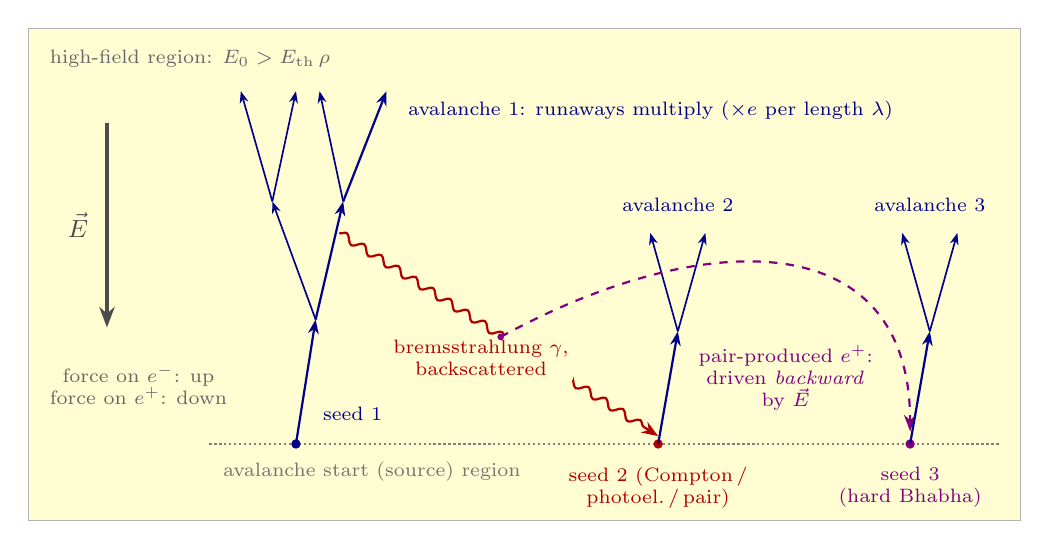
\begin{tikzpicture}[x=1cm, y=1cm,
      elec/.style={-{Stealth[length=1.8mm]}, thick, blue!55!black},
      elecb/.style={-{Stealth[length=1.5mm]}, semithick, blue!55!black},
      photon/.style={-{Stealth[length=2.1mm]}, thick, red!70!black,
        decorate, decoration={snake, amplitude=0.5mm, segment length=2.6mm,
        post length=2mm}},
      posi/.style={-{Stealth[length=2.1mm]}, thick, dashed, violet},
      lab/.style={font=\scriptsize, align=center}
    ]
    % high-field region
    \fill[yellow!18] (0,-0.35) rectangle (12.6,5.9);
    \draw[black!30] (0,-0.35) rectangle (12.6,5.9);
    \node[lab, anchor=north west, text=black!60] at (0.15,5.75)
      {high-field region: $E_0 > E_{\mathrm{th}}\,\rho$};

    % E field arrow + forces
    \draw[-{Stealth[length=2.6mm]}, very thick, black!70]
      (1.0,4.7) -- (1.0,2.1) node[midway, left=1mm, font=\small] {$\vec E$};
    \node[lab, text=black!60, anchor=north] at (1.4,1.75)
      {force on $e^-$: up\\force on $e^{+}$: down};

    % source region
    \draw[densely dotted, thick, black!50] (2.3,0.62) -- (12.35,0.62);
    \node[lab, anchor=south west, text=black!55] at (2.35,0.02)
      {avalanche start (source) region};

    % avalanche 1
    \coordinate (s1) at (3.4,0.62);
    \fill[blue!55!black] (s1) circle (1.7pt);
    \node[lab, blue!55!black, anchor=west] at (3.62,1.0) {seed 1};
    \draw[elec]  (s1) -- (3.65,2.2);
    \draw[elec]  (3.65,2.2) -- (4.0,3.7);
    \draw[elecb] (3.65,2.2) -- (3.1,3.7);
    \draw[elecb] (4.0,3.7)  -- (3.7,5.1);
    \draw[elec]  (4.0,3.7)  -- (4.55,5.1);
    \draw[elecb] (3.1,3.7)  -- (2.7,5.1);
    \draw[elecb] (3.1,3.7)  -- (3.4,5.1);
    \node[lab, blue!55!black, anchor=west] at (4.7,4.85)
      {avalanche 1: runaways multiply ($\times e$ per length $\lambda$)};

    % backward photon -> seed 2
    \draw[photon] (3.95,3.3) -- (8.0,0.72);
    \node[lab, red!70!black, anchor=north, fill=yellow!18, inner sep=1.5pt]
      at (5.75,2.0) {bremsstrahlung $\gamma$,\\backscattered};
    \fill[red!70!black] (8.0,0.62) circle (1.7pt);
    \node[lab, red!70!black, anchor=north] at (8.0,0.45)
      {seed 2 (Compton\,/\\photoel.\,/\,pair)};
    \draw[elec]  (8.0,0.62) -- (8.25,2.05);
    \draw[elecb] (8.25,2.05) -- (7.9,3.3);
    \draw[elecb] (8.25,2.05) -- (8.6,3.3);
    \node[lab, blue!55!black, anchor=south] at (8.25,3.45) {avalanche 2};

    % backward positron -> seed 3: born ON the photon path (pair production
    % is a PHOTON channel; hanging this off an electron track would draw
    % trident production, which the engine does not implement)
    \fill[violet] (6.0,1.98) circle (1.2pt);
    \draw[posi] (6.0,1.98) .. controls (8.6,3.4) and (11.2,3.4) .. (11.2,0.78);
    \node[lab, violet, anchor=north] at (9.62,2.0)
      {pair-produced $e^{+}$:\\driven \emph{backward}\\by $\vec E$};
    \fill[violet] (11.2,0.62) circle (1.7pt);
    \node[lab, violet, anchor=north] at (11.2,0.45)
      {seed 3\\(hard Bhabha)};
    \draw[elec]  (11.2,0.62) -- (11.45,2.05);
    \draw[elecb] (11.45,2.05) -- (11.1,3.3);
    \draw[elecb] (11.45,2.05) -- (11.8,3.3);
    \node[lab, blue!55!black, anchor=south] at (11.45,3.45) {avalanche 3};
  \end{tikzpicture}
  \caption{The relativistic feedback loop (Dwyer) the model is built to
  capture. A seed electron runs away and multiplies into avalanche~1. Some
  of its bremsstrahlung photons propagate or Compton-backscatter
  \emph{against} the avalanche direction and liberate fresh energetic
  electrons near the start region; positrons pair-produced by those photons
  carry positive charge and are therefore accelerated \emph{backward} by the
  same field, seeding further electrons through hard Bhabha collisions. If each
  avalanche seeds on average at least one successor, the discharge is
  self-sustaining.}
  \label{fig:feedback}
\end{figure}

Modeling this therefore needs three coupled ingredients:

\begin{enumerate}
  \item \textbf{High-energy particle transport} (electrons, photons,
  positrons, $\gtrsim$~keV--MeV--GeV): individual particles pushed through
  air with Monte Carlo collisions. Photons and positrons get the same
  first-class treatment as electrons precisely because they carry the
  relativistic feedback.
  \item \textbf{A low-energy plasma fluid} (electrons below a cutoff,
  positive and negative ions): far too numerous to track as particles;
  represented as densities on the mesh, evolving by attachment,
  recombination, and drift, and producing a conductivity $\sigma$.
  \item \textbf{Self-consistent field feedback}: the electric field is the
  imposed thundercloud profile \emph{relaxed} by the conductivity and by the
  space charge of both populations.
\end{enumerate}

The RREA model implements (1) as a WarpX particle extension, (2) and (3) as
a native AMReX library, and couples them inside the WarpX time step. The
simulation geometry is cylindrical RZ (radius $r$, altitude $z$), which
matches the natural symmetry of a vertical avalanche column.

%=====================================================================
\section{The Building Blocks: AMReX and WarpX in Five Minutes}\label{sec:blocks}

\subsection{AMReX}

\href{https://amrex-codes.github.io}{AMReX} is a C++ framework for
block-structured mesh codes. The concepts used constantly in this project:

\begin{itemize}
  \item \textbf{Box / BoxArray}: the rectangular index space of the mesh is
  chopped into boxes (here up to $64\times64$ cells, set by
  \code{amr.max\_grid\_size}). Boxes are the unit of parallel distribution.
  \item \textbf{DistributionMapping}: assigns each box to one MPI rank.
  \item \textbf{MultiFab}: ``multiple FArrayBoxes'' (Fortran array
  boxes) --- \emph{the}
  AMReX data structure: one floating-point field (e.g.\ electron density)
  stored box-by-box across all ranks, with ghost cells for stencils. The fluid,
  charge, and WarpX-facing field arrays are MultiFabs; the Maxwell update uses
  a replicated staggered state assembled from them.
  \item \textbf{ParticleContainer}: distributed particle storage; each
  particle carries position, momentum, a statistical \emph{weight}
  (how many real particles one computational ``macroparticle'' represents),
  and optional extra components.
\end{itemize}

\subsection{WarpX}

\href{https://ecp-warpx.github.io}{WarpX} is an electromagnetic/electrostatic
particle-in-cell (PIC) code built on AMReX. A PIC code advances plasma in a
loop: deposit particle charge onto the mesh $\to$ solve for fields $\to$
interpolate (``gather'') fields to particles $\to$ push particles. WarpX
provides, ready-made:

\begin{itemize}
  \item the RZ cylindrical geometry and distributed particle storage;
  \item named particle species defined in a text input deck
  (\code{particles.species\_names = ...}), each backed by a
  ParticleContainer;
  \item the main time loop (\code{WarpXEvolve.cpp}), field containers,
  I/O, checkpointing scaffolding, and MPI orchestration;
  \item an electrostatic solver, \code{ComputeSpaceChargeField}, which the
  RREA model \emph{replaces} (Section~\ref{sec:hooks}).
\end{itemize}

The project gitlinks pin \textbf{WarpX 26.06} and \textbf{AMReX 26.06} in
protected archival forks. AMReX is built from source inside the WarpX build;
the executable is RZ, double precision, MPI+OpenMP.

The key idea to keep in mind: \emph{WarpX supplies particles, mesh, and the
time loop; the RREA code supplies the physics of air and the field solver,
and inserts itself at a few precisely chosen points of the loop.}

%=====================================================================
\section{The Big Picture: Overlay + Native Library}\label{sec:overlay}

The protected forks archive pristine release commits; this repository carries
no modified copy of either framework. The RREA implementation consists of two
parts:

\begin{description}
  \item[Native library] A standalone static library
  (\code{rrea\_amrex\_field\_solver}; sources in
  \path{native_amrex_rrea/src} and \path{native_amrex_rrea/include/rrea/}) that depends
  only on AMReX --- not on
  WarpX. It contains the fluid state, the Maxwell advance, the field
  initializer and atmosphere profile, the interaction-table loader,
  the seed schedule, and the event accumulator. Because it has no WarpX
  dependency, this physics can be built and tested without constructing
  WarpX. Focused MPI variants additionally exercise distributed invariants.
  \item[WarpX overlay]
  (\path{native_amrex_rrea/warpx_overlay/Source/Rrea})
  The WarpX-aware kinetic-transport and coupling layer. It owns the particle
  loops and their shared final-state primitives, links the native library, and
  is copied into a WarpX source tree at build time.
\end{description}

\begin{center}
\begin{tabular}{@{}>{\raggedright\arraybackslash}p{0.45\textwidth}>{\raggedright\arraybackslash}p{0.47\textwidth}@{}}
\toprule
\textbf{Native library (AMReX only)} & \textbf{Overlay (WarpX-aware transport/coupling)} \\
\midrule
\code{LowEnergyFluidState} & \code{RreaParticleInteraction} (MC engine) \\
\code{RreaAmrexAdvance} & \code{TransportStep} (the four species phases) \\
\code{RreaFieldInitializer}, \code{RreaAltitudeProfile} & \code{RreaRng}
(counter-based RNG) \\
\code{RreaInteractionTables} (schema-6 loader) & checkpoint rank-state
helpers \\
\code{RreaEventAccumulator}, \code{RreaSeedSchedule} & \\
\bottomrule
\end{tabular}
\end{center}

\begin{figure}[H]
  \centering
  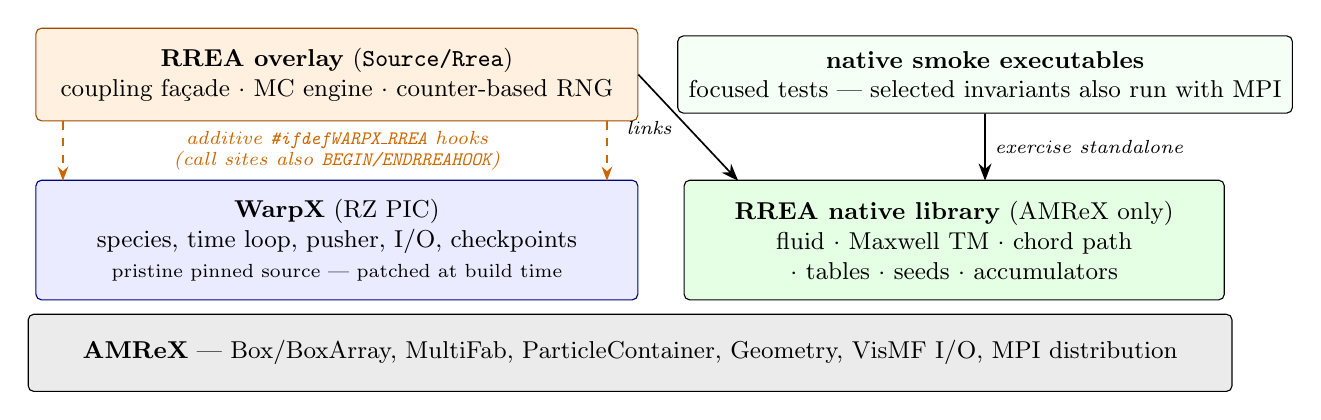
\begin{tikzpicture}[
      scale=0.98, transform shape,
      layer/.style={draw, rounded corners=2pt, align=center, font=\small,
                    inner sep=4pt},
      lab/.style={font=\scriptsize\itshape, align=center},
      arr/.style={-{Stealth[length=2.2mm]}, semithick},
      hook/.style={-{Stealth[length=1.8mm]}, semithick, dashed,
                   orange!80!black}
    ]
    \node[layer, fill=black!8, minimum width=15.6cm, minimum height=1.0cm]
      (amrex) at (0,0)
      {\textbf{AMReX} --- Box/BoxArray, MultiFab, ParticleContainer,
       Geometry, VisMF I/O, MPI distribution};
    \node[layer, fill=warpxfill, draw=warpxedge, minimum width=7.8cm, minimum height=1.55cm,
          anchor=south] (warpx) at (-3.8,0.68)
      {\textbf{WarpX} (RZ PIC)\\
       species, time loop, pusher, I/O, checkpoints\\
       {\scriptsize pristine pinned source --- patched at build time}};
    \node[layer, fill=nativefill, minimum width=7.0cm, minimum height=1.55cm,
          anchor=south] (native) at (4.2,0.68)
      {\textbf{RREA native library} (AMReX only)\\
       fluid $\cdot$ Maxwell TM $\cdot$ chord path\\
       $\cdot$ tables $\cdot$ seeds $\cdot$ accumulators};
    \node[layer, fill=rreafill, draw=rreaedge, minimum width=7.8cm, minimum height=1.2cm,
          anchor=south] (overlay) at (-3.8,3.0)
      {\textbf{RREA overlay} (\code{Source/Rrea})\\
       coupling fa\c{c}ade $\cdot$ MC engine $\cdot$ counter-based RNG};
    \node[layer, fill=green!4, minimum width=6.2cm, minimum height=1.0cm,
          anchor=south] (smoke) at (4.6,3.1)
      {\textbf{native smoke executables}\\
       focused tests --- selected invariants also run with MPI};
    % additive hooks (every insertion #ifdef-guarded; only the call sites
    % also carry BEGIN/END markers)
    \foreach \x in {-7.35,-0.3}
      \draw[hook] (\x,3.0) -- (\x,2.23);
    \node[lab, orange!80!black, align=center] at (-3.8,2.62)
      {additive \code{\#ifdef WARPX\_RREA} hooks\\
       (call sites also \code{BEGIN/END RREA HOOK})};
    % overlay links native
    \draw[arr] (overlay.east) -- node[lab, pos=0.5, left=2.5pt] {links}
      (1.4,2.23);
    % smokes exercise native
    \draw[arr] (smoke.south) -- node[lab, right] {exercise standalone}
      (4.6,2.23);
  \end{tikzpicture}
  \caption{Where each piece of code sits. WarpX and the RREA native
  library both stand directly on AMReX; the overlay is the only
  WarpX-aware code and is grafted onto a pristine WarpX tree at build time
  through guarded, exact-match, idempotent patches (Section~\ref{sec:hooks}).
  The native library is exercised standalone by the native smoke executables
  before it ever runs inside WarpX; the production executable
  \code{warpx.rz} links all of it into one binary.}
  \label{fig:stack}
\end{figure}

This split follows dependency ownership (Figure~\ref{fig:stack}): AMReX-only
mesh, field and table code lives in the native library; WarpX particle
transport and coupling live in the overlay. Header primitives keep much of the
transport physics independently testable without running WarpX.

%=====================================================================
\section{How the Code Attaches to WarpX}
\label{sec:hooks}

\subsection{The source-preparation step}

A pristine WarpX checkout is never edited by hand. The script
\path{scripts/prepare_rrea_warpx_source.py} builds the combined source
tree:

\begin{enumerate}
  \item copies the pristine WarpX tree to a build location (it refuses to
  run in-place);
  \item copies the overlay directory in as \code{Source/Rrea};
  \item applies a small set of guarded patches to stock WarpX
  files. Every insertion is \code{\#ifdef WARPX\_RREA}-guarded; each
  call-site hook is additionally wrapped in
  \code{// BEGIN RREA HOOK ... // END RREA HOOK} comments. Each patch is
  applied by an exact-match text search (``needle''). The patch operations are
  idempotent, so \code{--refresh} can update an existing prepared tree; if a
  WarpX update moves a needle, the script \emph{aborts} instead of guessing.
\end{enumerate}

The patches add guarded declarations and calls without deleting stock behavior. The full
list of patched files:

\begin{center}
\begin{tabular}{@{}>{\raggedright\arraybackslash}p{0.42\textwidth}>{\raggedright\arraybackslash}p{0.52\textwidth}@{}}
\toprule
\textbf{WarpX file} & \textbf{What the patch adds} \\
\midrule
\path{CMakeLists.txt} & \path{add_subdirectory(Source/Rrea)}; overlay
sources join the WarpX library target with \code{WARPX\_RREA=1}. \\
\addlinespace
\path{Source/WarpX.H} & a \code{SpaceChargeSolvePurpose} enum and a
\code{purpose} parameter on \code{ComputeSpaceChargeField}, so the hook can
distinguish initialization solves from evolution solves. \\
\addlinespace
\path{Source/FieldSolver/WarpXSolveFieldsES.cpp} & \textbf{the field-solver
replacement}: at the top of \code{ComputeSpaceChargeField}, call
\path{RreaWarpXCoupling::BeforeFieldSolve(...)}; if it returns true, WarpX's
own electrostatic solve is skipped entirely. \\
\addlinespace
\path{Source/Evolve/WarpXEvolve.cpp} & three calls in the step loop:
\code{InjectScheduledSeeds} (before the push),
\code{CaptureRreaPositionsBeforePush} (just before \code{OneStep}), and
\code{AfterParticlePushBeforeBoundaries} (just after). \\
\addlinespace
\path{Source/Initialization/WarpXInitData.cpp} & tags the startup field
solve with \code{Initialization} purpose. \\
\addlinespace
\path{Source/Diagnostics/FlushFormats/FlushFormatCheckpoint.cpp} /
\path{Source/Diagnostics/WarpXIO.cpp} & write/read the extra
RREA checkpoint payload alongside WarpX's own checkpoint. \\
\bottomrule
\end{tabular}
\end{center}

\subsection{The ordering contract}

The physics is only correct if the hooks run in a specific order inside one
step (Figure~\ref{fig:steporder}): \emph{inject seeds $\to$ snapshot particle
state $\to$ stock WarpX step $\to$ RREA trajectory reconstruction and air
transport $\to$ WarpX boundary handling $\to$ RREA field solve}. The
preparation script literally asserts
this ordering when patching \code{WarpXEvolve.cpp}: if a future WarpX
version reorders its loop, source preparation fails loudly instead of
silently producing wrong physics.

The order is a physics contract, not a convenient insertion point. RREA must
see the pushed chord \emph{while an escaping parent still exists}: a particle
that leaves the domain this step still traveled its chord through air inside
it, and WarpX's boundary handling would delete it first. At the other end,
generic resampling must not run before the atomic secondary groups have been
committed --- which is why the asserted anchors include WarpX's own
\code{doResampling}, a stage that runs inside the protected window and is not
drawn in Figure~\ref{fig:steporder}. This ``fail-closed'' habit --- abort
rather than improvise --- recurs everywhere in the project
(Section~\ref{sec:failclosed}).

\begin{figure}[H]
  \centering
  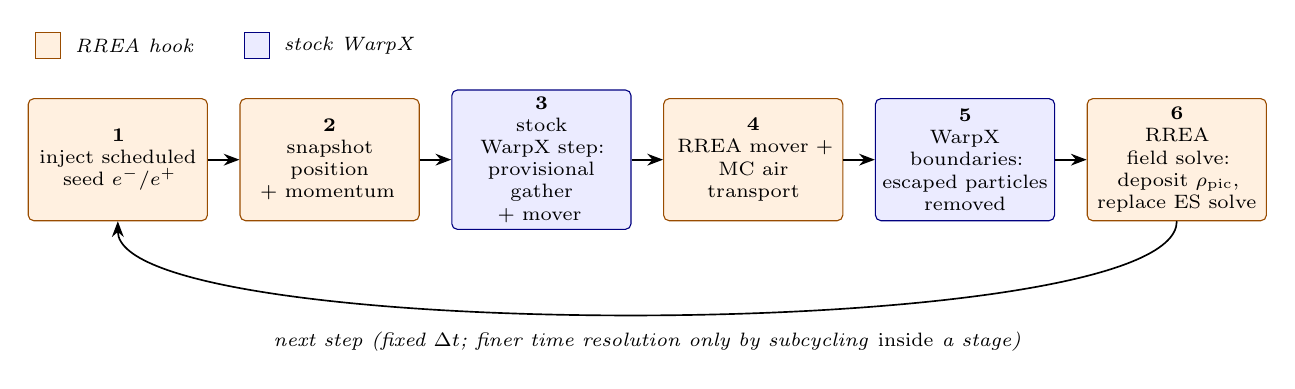
\begin{tikzpicture}[
      stepbox/.style={draw, rounded corners=2pt, align=center, font=\scriptsize,
                   minimum height=1.55cm, text width=2.1cm, inner sep=2.5pt},
      rr/.style={stepbox, fill=rreafill, draw=rreaedge},
      wx/.style={stepbox, fill=warpxfill, draw=warpxedge},
      arr/.style={-{Stealth[length=2mm]}, semithick},
      lab/.style={font=\scriptsize\itshape, align=center}
    ]
    \node[rr] (s1) at (0,0)
      {\textbf{1}\\ inject scheduled\\ seed $e^-/e^+$};
    \node[rr, right=0.4cm of s1] (s2)
      {\textbf{2}\\ snapshot position\\ $+$ momentum};
    \node[wx, right=0.4cm of s2] (s3)
      {\textbf{3}\\ stock WarpX step:\\ provisional gather\\ $+$ mover};
    \node[rr, right=0.4cm of s3] (s4)
      {\textbf{4}\\ RREA mover $+$\\ MC air transport};
    \node[wx, right=0.4cm of s4] (s5)
      {\textbf{5}\\ WarpX boundaries:\\ escaped particles\\ removed};
    \node[rr, right=0.4cm of s5] (s6)
      {\textbf{6}\\ RREA field solve:\\ deposit $\rho_{\mathrm{pic}}$,\\ replace ES solve};
    \foreach \a/\b in {s1/s2, s2/s3, s3/s4, s4/s5, s5/s6}
      \draw[arr] (\a) -- (\b);
    \draw[arr] (s6.south) to[out=-90, in=-90, looseness=0.3]
      node[lab, below=1mm, midway]
      {next step (fixed $\Delta t$; finer time resolution only by
       subcycling \emph{inside} a stage)} (s1.south);
    % legend
    \node[draw=rreaedge, fill=rreafill, minimum width=3.2mm, minimum height=3.2mm,
          inner sep=0, anchor=west] (lg1) at (-1.05,1.45) {};
    \node[lab, anchor=west] at (lg1.east) {\,RREA hook};
    \node[draw=warpxedge, fill=warpxfill, minimum width=3.2mm, minimum height=3.2mm,
          inner sep=0, anchor=west] (lg2) at (1.6,1.45) {};
    \node[lab, anchor=west] at (lg2.east) {\,stock WarpX};
  \end{tikzpicture}
  \caption{The per-step ordering contract. Orange stages are RREA hooks;
  blue stages are stock WarpX. The source-preparation script asserts
  this sequence --- plus WarpX's own \code{doResampling} between stages 4
  and 5, not drawn --- when patching \code{WarpXEvolve.cpp}, and aborts if
  a WarpX update reorders its loop. The numbers match the walkthrough in
  Section~\ref{sec:step}.}
  \label{fig:steporder}
\end{figure}

%=====================================================================
\section{Species and the Input Deck}\label{sec:deck}

The model manages three WarpX species, declared in a completely ordinary
WarpX input deck (template:
\path{cases/rrea/production/inputs}):

\begin{verbatim}
particles.species_names = rrea_electrons rrea_photons rrea_positrons
rrea_electrons.species_type = electron
rrea_photons.species_type   = photon
rrea_positrons.species_type = positron
\end{verbatim}

All three use \code{injection\_style = none}: WarpX never injects these
particles itself. The RREA code owns creation and physical terminal decisions;
WarpX's boundary pass removes escaped slots afterward. At startup the coupling verifies that each named species really has the
mass/charge it expects and that the three names are distinct --- another
fail-closed check.

Everything else the model needs arrives as \code{rrea.*} input parameters.
The important groups:

\begin{center}
\begin{tabular}{@{}>{\raggedright\arraybackslash}p{0.30\textwidth}>{\raggedright\arraybackslash}p{0.64\textwidth}@{}}
\toprule
\textbf{Group} & \textbf{Representative parameters} \\
\midrule
Ownership & \path{rrea.enable=1} and
\path{rrea.field_model=maxwell_rz_yee_material_coupled}. External
particle fields are forbidden --- the field may come only from the RREA
solver. \\
\addlinespace
Transport tables & \path{rrea.interaction_table_config} (path),
\path{rrea.transport_model} (exact string match against the transport configuration);
photon feedback and positron transport are unconditional and have no deck
keys --- the table loader aborts unless the transport configuration declares
both enabled. Optical-depth guards
(\path{rrea.transport_max_optical_depth_per_substep},
\path{rrea.transport_max_subcycles}, \path{rrea.transport_strict_guards=1}). \\
\addlinespace
Population control & \path{rrea.population_ceiling_policy=adaptive_resample_v1}
(mechanism and the scope of its unbiasedness in \S\ref{sec:failclosed}) with
\path{rrea.population_target_electron_macros}, \path{rrea.max_electron_macros},
\path{rrea.max_photon_macros}, \path{rrea.max_positron_macros} as fail-closed backstops
above the control band; \path{strict_abort_v1} is the engine default and the
policy of an explicit reference run; \path{rrea.low_energy_cutoff_eV} overrides
the bundle's charged floor for a study (\S\ref{sec:model-scope}). \\
\addlinespace
Field / Maxwell & \path{rrea.acceleration_field_v_per_m},
\path{rrea.acceleration_z_max_m} (imposed profile), mesh spacing and timestep. \\
\addlinespace
Atmosphere & \path{rrea.air_density_model} (a constant density ratio at a
chosen altitude, or a full altitude profile), the density ratio
$\rho/\rho_0$ itself. The air composition is fixed by the tables' G4\_AIR
reference, not by deck fractions. See
Section~\ref{sec:density} for how one table set serves every altitude. \\
\addlinespace
Seeding & \path{rrea.seed_schedule_path} (a CSV of when/where/how many
seed electrons and positrons appear, at what energy, weight, and
direction; the optional \code{species\_id} column routes each event to its
container), \path{rrea.rng_seed}. The production default schedule is the
PARMA cosmic-ray $e^-$/$e^+$ source with its $t=0$ stationary bath
(\S\ref{sec:module-index}, Deposition and population); the mono-1-MeV pulse and the
C\&D cohort remain selectable through
\path{config/rrea_defaults.json} / the driver. \\
\addlinespace
Diagnostics & \path{rrea.diag_interval}, \path{rrea.output_dir},
\path{rrea.video_diag_*} (Section~\ref{sec:diag}). \\
\bottomrule
\end{tabular}
\end{center}

The \emph{macroparticle weight} deserves a beginner's note: one
computational particle represents $w$ real particles ($w$ is set by the
seed schedule; secondaries inherit the parent scale). Larger $w$ means
fewer macros (cheaper, noisier), smaller $w$ the reverse.

One more setting a newcomer should know about: the \emph{time step} is
fixed for the whole run (\code{warpx.const\_dt}). There is no adaptive global
stepping --- wherever finer time
resolution is needed, the relevant layer subcycles internally (the Monte
Carlo transport under its optical-depth guard; the coupled fluid/Maxwell
advance under its conductivity, diffusion and drift limits), keeping the
outer step sequence shared by every coupled subsystem and checkpoint.

%=====================================================================
\section{One Time Step, Start to Finish}
\label{sec:step}

Figure~\ref{fig:dataflow} shows the whole per-step data flow at a glance;
the numbered walkthrough below follows the same arrows in execution order.

\begin{figure}[H]
  \centering
  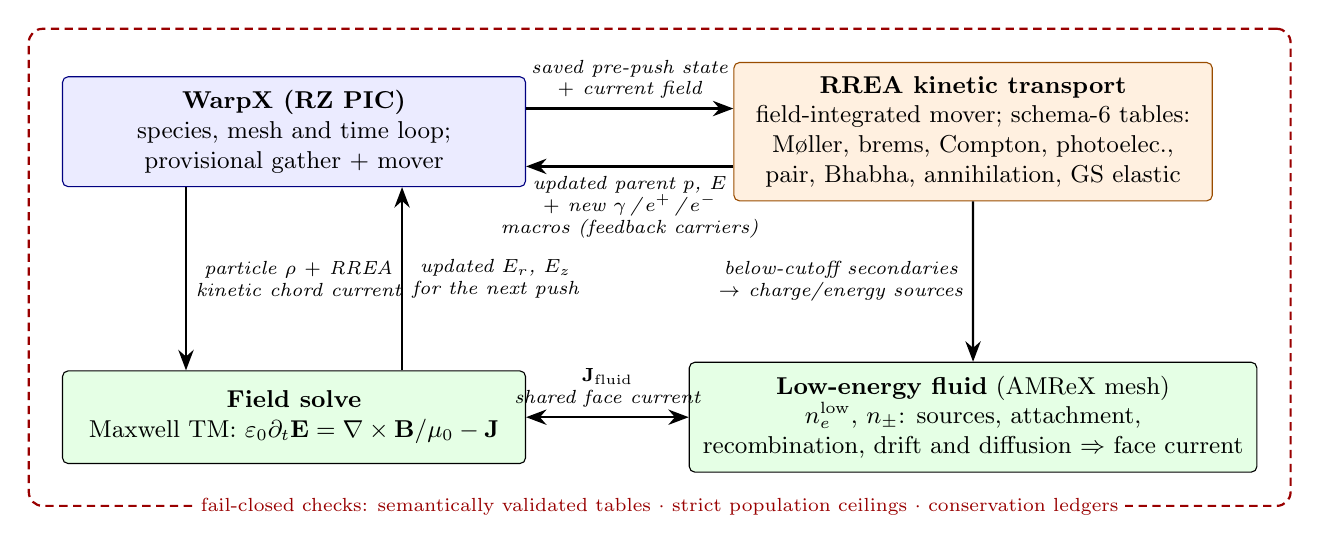
\begin{tikzpicture}[
      scale=0.98, transform shape,
      box/.style={draw, rounded corners=2pt, align=center, inner sep=5pt,
                  font=\small, minimum height=1.2cm},
      lab/.style={font=\scriptsize\itshape, align=center},
      arr/.style={-{Stealth[length=2.6mm]}, thick}
    ]
    \node[box, fill=warpxfill, draw=warpxedge, minimum width=6.0cm] (warpx) at (0,0)
      {\textbf{WarpX (RZ PIC)}\\
       species, mesh and time loop;\\
       provisional gather $+$ mover};
    \node[box, fill=rreafill, draw=rreaedge, minimum width=6.2cm] (mc) at (8.8,0)
      {\textbf{RREA kinetic transport}\\
       field-integrated mover; schema-6 tables:\\
       M{\o}ller, brems, Compton, photoelec.,\\
       pair, Bhabha, annihilation, GS elastic};
    \node[box, fill=nativefill, minimum width=6.2cm] (fluid) at (8.8,-3.7)
      {\textbf{Low-energy fluid} (AMReX mesh)\\
       $n_e^{\mathrm{low}}$, $n_\pm$: sources, attachment,\\
       recombination, drift and diffusion $\Rightarrow$ face current};
    \node[box, fill=nativefill, minimum width=6.0cm] (field) at (0,-3.7)
      {\textbf{Field solve}\\
       Maxwell TM: $\varepsilon_0\partial_t\mathbf{E}
       =\nabla\times\mathbf{B}/\mu_0-\mathbf{J}$};

    \draw[arr] ([yshift=3mm]warpx.east) -- node[lab, above]
      {saved pre-push state\\$+$ current field} ([yshift=3mm]mc.west);
    \draw[arr] ([yshift=-4.5mm]mc.west) -- node[lab, below]
      {updated parent $p$, $E$\\$+$ new $\gamma$\,/\,$e^+$\,/\,$e^-$\\macros
       (feedback carriers)}
      ([yshift=-4.5mm]warpx.east);
    \draw[arr] (mc) -- node[lab, left]
      {below-cutoff secondaries\\$\to$ charge/energy sources} (fluid);
    \draw[{Stealth[length=2.6mm]}-{Stealth[length=2.6mm]}, thick]
      (fluid) -- node[lab, above]
      {$\mathbf{J}_{\mathrm{fluid}}$\\shared face current}
      (field);
    \draw[arr] ([xshift=-14mm]warpx.south) -- node[lab, right]
      {particle $\rho$ $+$ RREA\\kinetic chord current} ([xshift=-14mm]field.north);
    \draw[arr] ([xshift=14mm]field.north) -- node[lab, right]
      {updated $E_r$, $E_z$\\for the next push} ([xshift=14mm]warpx.south);

    \node[draw=red!60!black, densely dashed, thick, rounded corners=5pt,
          inner sep=12pt, fit=(warpx)(mc)(fluid)(field)] (frame) {};
    \node[font=\scriptsize, red!60!black, fill=white, inner sep=2.5pt,
          align=center] at (frame.south)
      {fail-closed checks: semantically validated tables $\cdot$ strict
       population ceilings $\cdot$ conservation ledgers};
  \end{tikzpicture}
  \caption{Per-step data flow. WarpX executes its stock step provisionally;
  the RREA engine reconstructs the physical trajectories from the saved state,
  applies air physics, and overwrites the endpoints, promoting above-cutoff secondaries to new
  macroparticles --- which closes Dwyer's relativistic feedback loop ---
  and demoting below-cutoff secondaries into the low-energy fluid; the
  fluid and kinetic chord currents drive the Maxwell TM update, whose field
  feeds the next particle push. The dashed frame is
  the fail-closed checks around the coupled path
  (Section~\ref{sec:failclosed}); the execution order within one step is
  the hook sequence of Figure~\ref{fig:steporder}.}
  \label{fig:dataflow}
\end{figure}

All coupling state lives in one singleton,
\path{rrea::warpx::RreaWarpXCoupling}, declared in
\path{native_amrex_rrea/warpx_overlay/Source/Rrea/RreaWarpXCoupling.H}.  Its members are
defined across sibling translation units, one responsibility each: the field
step (\path{RreaWarpXCoupling.cpp}), startup contracts and table/schedule
loading (\path{RreaCouplingConfig.cpp}), population control
(\path{RreaCouplingPopulation.cpp}), seed and event sources
(\path{RreaCouplingSources.cpp}), the reduced CSV
(\path{RreaCouplingDiagnostics.cpp}), video frames
(\path{RreaCouplingVideoFrame.cpp}), the C\&D plane stream
(\path{RreaCouplingPlaneWriter.cpp}), checkpoint/rank-state I/O
(\path{RreaCouplingCheckpoint.cpp}) and the charge-continuity fixture
(\path{RreaActualContinuityFixture.cpp}). Shared helpers sit in
\path{RreaCouplingDetail.H}; the one rank-local sweep over live macroparticles
(\code{RreaForEachValidParticle}, \path{RreaParticleSweep.H}) gives the
soft-deleted-slot guard a single owner.
Its per-step entry points fire in this order:

\begin{enumerate}
  \item \textbf{\code{InjectScheduledSeeds}} --- reads the seed-schedule CSV
  and creates any seed macros whose injection time falls in this step,
  routed by the schedule's \code{species\_id} into the
  \code{rrea\_electrons} or \code{rrea\_positrons} container.

  \item \textbf{\code{CaptureRreaPositionsBeforePush}} --- copies every
  managed particle's position \emph{and momentum} into extra particle
  components (\code{rrea\_prev\_*}): the pre-push state the transport
  below re-integrates from.

  \item \textbf{WarpX \code{OneStep}} --- the stock WarpX gather and
  relativistic push still execute, but the kick is \emph{discarded}: the
  engine rebuilds direction, energy and geometry from the captured
  pre-push state, drives its own running chord with the field impulse
  re-applied per substep (Strang split, Gauss--Legendre line-integral
  work), and overwrites WarpX's endpoint with the point the particle
  actually reached.  \code{algo.particle\_pusher} is therefore inert
  plumbing; \code{algo.particle\_shape} is \emph{not} (the hook's own
  charge deposition uses it).

  \item \textbf{\code{AfterParticlePushBeforeBoundaries}} --- the material
  physics. For each managed particle, the Monte Carlo engine
  (\code{RreaParticleInteraction::Apply}) drives the running chord
  through air from the pre-push state. \code{Apply} only builds the per-step
  context (\code{TransportStep}, \path{RreaTransportStep.H}) and runs four
  phases, one translation unit each: the electron, photon and positron loops
  (\path{RreaElectronTransport.cpp}, \path{RreaPhotonTransport.cpp} and
  \path{RreaPositronTransport.cpp}), then the commit tail
  (\path{RreaSecondaryCommit.cpp} and \path{RreaNewbornAdvance.cpp}). The charged
  loops are separate by \emph{policy} only; the drag, elastic and final-state
  physics is shared (\path{RreaChargedFinalStates.H},
  \path{RreaPhotonFinalStates.H}, \path{RreaMaterialPath.H},
  \path{RreaPathFieldWork.H}). Along the chord:
  \begin{itemize}
    \item continuous energy loss (collisional + radiative drag) and
    field work are integrated along the chord;
    \item discrete interactions compete as hazards: the traversed
    \emph{optical depth} in each hard channel (M{\o}ller, bremsstrahlung,
    photon Compton / photoelectric / pair production, positron Bhabha /
    annihilation) is accumulated, and the engine samples which event, if any,
    occurs and where on the chord. Goudsmit--Saunderson elastic deflection is
    accumulated separately over each sub-interval;
    \item sampling uses the \textbf{schema-6 tables}
    (Section~\ref{sec:tables}) with log-log interpolation, local
    air-density scaling (Section~\ref{sec:density}), and
    \emph{forbidden} extrapolation;
    \item secondaries above the cutoffs become new macroparticles of the
    appropriate species; charged secondaries \emph{below} the cutoff
    are ``demoted'': their charge and energy are deposited into mesh
    accumulators as low-energy-electron and ion sources (cutoffs:
    \S\ref{sec:model-scope});
    \item every state-changing discrete interaction closes a charge and energy ledger;
    a violation aborts;
    \item randomness comes from a counter-based RNG keyed on the physical
    identity of the particle, so each particle's random stream does not depend
    on MPI layout;
    \item before any group of new particles is committed, all ranks plan
    exact-CIC control over survivors plus staged charged candidates, then
    collectively preflight both charged plans and all population ceilings
    (Section~\ref{sec:failclosed}).
  \end{itemize}

  \item \textbf{WarpX boundary handling} --- stock
  WarpX removes particles that left the domain.

  \item \textbf{\code{BeforeFieldSolve}} --- called where WarpX would solve
  its electrostatic field; returns \code{true}, so WarpX's solver never
  runs. Instead:
  \begin{itemize}
    \item the hook deposits the energetic particles' charge itself --- in the
    electrostatic branch stock WarpX pushes with deposition skipped, because
    the stock design deposits inside the very solver this hook replaces;
    \item the accumulated event sources (low-energy electrons, positive and
    direct negative ions, ionization energy) are normalized and handed to
    the fluid;
    \item \code{RreaAmrexAdvance::AdvanceOneStep} evolves the fluid and the
    field (Section~\ref{sec:field});
    \item the resulting $E_r, E_z$ are copied back into WarpX's field
    MultiFabs (so the next step's particle push feels the updated field);
    \item video frames and the reduced diagnostics row are written if due.
  \end{itemize}
\end{enumerate}

%=====================================================================
\section{The Schema-6 Interaction Tables}
\label{sec:tables}

Process rates and several energy/final-state distributions come from
pre-generated data compared with Geant4 10.7.4 and organized under
\path{rrea_transport_tables/}. Runtime analytic models remain explicit where
used (notably free Klein--Nishina Compton and bounded Modified--Tsai bremsstrahlung
angles). The table directory is selected through \path{transport_physics.json}
and the loader checks units, ranges and cutoffs; focused tests compare the
physical holdouts.

The shared electron/positron brems angle uses the Modified--Tsai distribution
of \code{G4ModifiedTsai} in the pinned Geant4 source: its Gamma-mixture variable
$u$ is conditioned on $0\leq u\leq2\gamma$, then mapped by
$\cos\theta=1-u^2/(2\gamma^2)$, where $\gamma=1+K/(m_ec^2)$.
This analytic angle is independent of the tabulated photon energy; it does
not claim option-4's energy--angle correlation. It requires no angular table.

\begin{itemize}
  \item \textbf{Electrons}: restricted collisional drag, radiative and
  soft-radiative drag, hard M{\o}ller mean free path + secondary spectrum,
  bremsstrahlung MFP + photon energy CDF + analytic emission angles,
  Goudsmit--Saunderson elastic multiple-scattering angle CDFs;
  \item \textbf{Photons}: modeled-channel interaction MFP and probabilities,
  photoelectric subshell CDFs (with binding energies),
  nuclear and triplet pair production with Geant4 energy-sharing CDFs.
  Compton is the one channel whose final state is \emph{not} tabulated: its
  rate carries Geant4's incoherent scattering function (measured
  $-4.4$\,\% against free Klein--Nishina at 50\,keV), but the scattering
  angle is sampled at runtime from analytic free-electron Klein--Nishina;
  \item \textbf{Positrons}: \emph{restricted} collision stopping (numerically
  equal to the electron restricted table to $0.3\,\%$), soft-radiative drag,
  hard Bhabha, positron bremsstrahlung, in-flight and at-rest annihilation.
\end{itemize}

The photon and positron channels are what close the relativistic feedback
loop, and the engine makes that unconditional: every \emph{explicitly
produced} bremsstrahlung photon is a tracked particle able to Compton-scatter
or pair-produce anywhere in the domain (including \emph{behind} the avalanche
front), and pair-produced positrons --- which the ambient field accelerates
backward --- are transported with their own drag, hard-Bhabha, bremsstrahlung
and annihilation physics. There are no deck keys for either
(\S\ref{sec:deck}), so feedback is not a bolted-on approximation (no
``feedback factor''): it \emph{emerges} from the same per-particle Monte
Carlo transport as the primary avalanche.

Coherent Rayleigh scattering is deliberately excluded from the schema-6
kinetic gamma-ray transport: it has no runtime channel and no rate or angular
table. Near-cut photon mean free paths, angular transport, and feedback
predictions are conditional on that scope. This does not describe the separate
optical CloudScat calculation, whose atmospheric Rayleigh channel is enabled
unless explicitly disabled.

``Every explicitly produced'' is meant literally, and the qualifier matters.
Bremsstrahlung photons below the tracked cut are not created as particles at
all; they are carried as continuous radiative drag on the parent. That cut is
$k \geq \code{brems\_absolute\_cutoff\_eV}$, a flat energy declared by the
loaded transport configuration --- the engine binds to it and pins no value, so quote the
number from the bundle a result came from. Energy is conserved --- the sub-cutoff loss is
booked as \code{electron\_soft\_radiative\_stopping} and is correctly
\emph{not} converted into ion pairs --- but the photon \emph{count and
spectrum} are incomplete below the cut, where the tracked population is only
Compton-degraded photons. Any statement about photometer counts, low-energy
irradiance, or the backscattered feedback carriers (which pile up below
$m_ec^2/2 = 255$\,keV) must carry this caveat.

\subsection{One table set for every altitude: density scaling}
\label{sec:density}

The tables are computed once, for Geant4 \path{G4_AIR} at
$\rho_0=1.20479~\mathrm{kg/m^3}$ (dry air, 20\,\textdegree C, 1~atm), the
value the transport configuration records as \path{reference_density_kg_m3};
it is deliberately not called ``STP'', because the density at which the RREA
threshold and the reduced ion mobilities are quoted is a different one
(Section~\ref{sec:cdcheck}), and every ratio in the code names its reference.
But avalanches live at thundercloud altitudes where the air is
several times thinner --- so how can one table set be correct everywhere?
The answer is that as long as the \emph{composition} of the air is fixed
(the N$_2$/O$_2$ ratio of the tables' G4\_AIR reference), every interaction rate is
simply proportional to how many molecules a particle passes per meter.
The engine therefore evaluates the local density ratio
$\rho/\rho_0$ at each particle's position and rescales on the fly: mean
free paths stretch by $\rho_0/\rho$ (thinner air $=$ fewer collisions per
meter), while drags and other inverse lengths shrink by the same factor.
This rescaling is exact for every rate whose only density dependence is
that molecule count. The lone exception is the Sternheimer
density-effect term inside the collision stopping table, which stays
frozen at its $\rho_0$ value: it is identically zero below
$\approx$28\,MeV --- hence exactly zero at the $\approx$1.7\,MeV
friction minimum that sets the RREA threshold, so the threshold field
itself rescales exactly --- and reaches only $\approx$2.9\,\% by
100\,MeV, with the sign such that the drag is \emph{under}-estimated.

Where $\rho/\rho_0$ comes from is a deck choice
(\path{rrea.air_density_model}): either a single constant ratio for
explicit diagnostic inputs, or a full altitude profile ---
\code{RreaAltitudeProfile} in the native library interpolates a CSV of
density versus altitude, with the mesh's $z$ coordinate mapped to
altitude above sea level.  The canonical capture and all C\&D comparisons
use the realistic altitude profile, never a constant-density substitute.
The same profile machinery can shape the
imposed background field. The low-energy fluid follows suit: ion mobility
is density-scaled with the same ratio, and the electron mobility and
attachment are read from the source-anchored $E/N$ closure table, whose reduced
field carries that density, so the chemistry and conductivity are
consistent with the transport.

\subsection{Loading and integrity checks}

The loader (\code{rrea::RreaInteractionTables}, native library) validates the
tables semantically before transport mutates state: required files and columns,
units and ranges, monotone energy/CDF grids, finite positive rates, normalized
probabilities, cutoff agreement, and model identity. Any mismatch aborts the
run. Off-table energies are an error, not a clamp.
Schema-6 contains \emph{no} calibrated fudge factors. After validation
\code{Finalize()} resolves every table to a fixed \code{RreaTable} enum slot,
so the hot path indexes an array rather than looking a name up.

\subsection{Geant4-derived transport data and validation}

A natural beginner's question is why Geant4 is not called inside WarpX.
Geant4 is a full transport framework with its own geometry, stepping, and
threading model; embedding it in a PIC loop would be impractical. The project
therefore samples a versioned schema-6 table set produced from a declared Geant4
reference. Geant4 itself never executes inside WarpX.

The only production data tree is
\path{rrea_transport_tables/schema6/production/}, tracked in the repository as
RREATBL containers (\path{native_amrex_rrea/include/rrea/RreaTableContainer.H}): each file is a
JSON header naming every column with its dtype, over one deflate stream of
byte-shuffled float64 columns. \path{scripts/rrea_table_pack.py} writes them
and dumps any column back to CSV for review. Nothing is narrowed --- a float32
store would collapse the sub-ulp energy anchors the loader requires to stay
distinct. \path{transport_physics.json} stays plain text: it carries model
identifiers, cutoffs, acceptance tolerances and the path of every table, which
is where a replacement set is named.

At run time \code{RreaInteractionTables} loads the validated tables: a rate
such as ``mean free path of a 3.7~MeV electron against hard M{\o}ller
scattering'' is interpolated log-log between grid nodes, and when an
interaction fires its final state is drawn by inverting the appropriate CDF.

%=====================================================================
\section{The Low-Energy Fluid and the Field Solve}
\label{sec:field}

\subsection{Fluid state}

\code{rrea::LowEnergyFluidState} (native library) holds, per mesh cell:
low-energy electron density $n_e^{\mathrm{low}}$, positive and negative ion
densities $n_\pm$, their source rates (fed by the Monte Carlo demotions and
ionization), the conductivity $\sigma$, the local Maxwell relaxation time
$\tau_m = \varepsilon_0/\sigma$, and the fluid charge density. Each adaptive
material substep uses a symmetric half-reaction/transport--Maxwell/half-reaction
split.  The outer-step source-rate fields remain intact until the final half
reaction, so their known integral is distributed exactly across the substeps;
table attachment is re-evaluated after each updated field.  The transport stage computes
$\sigma = e \sum_s \mu_s\, n_s$ with mobilities scaled by air density, summed
only over carriers that are actually advanced (a species counted in $\sigma$
but held stationary would break charge continuity);
and drift the carriers with adaptive shared, $r$-weighted finite-volume
substeps using the committed donor-upwind face currents that enter the
corresponding Maxwell substeps.  The code
aborts on any substep whose multidimensional outgoing carrier CFL exceeds
the configured limit.

\subsection{Why the field solve is different from stock WarpX}

WarpX's electrostatic solver answers ``what field does this charge make?''
The thundercloud problem needs more: an \emph{imposed} background field
(the cloud's charging, held fixed as a boundary/reference state) that the
plasma progressively screens. The RREA solver therefore replaces that
electrostatic solve entirely with an explicit finite-speed update: the ambient
field is built once as a curl-free background (Section~\ref{sec:field-taper})
and the total field is then advanced by the RZ TM Maxwell equations
(Section~\ref{sec:field-maxwell}).

Screening is a consequence of that advance rather than a term in an operator.
Where the air has become conductive, the fluid's own committed face current
opposes the local field and the field relaxes on the Maxwell time
$\tau_m = \varepsilon_0/\sigma$ because Amp\`ere's law says it must.
Material continuity is a fail-closed outer-step gate and Gauss a monitor;
neither applies a correction.

\subsection{The Maxwell TM branch}
\label{sec:field-maxwell}

Every current here is poloidal, so under $m=0$ the complete retained field
content is the TM triplet $(E_r, E_z, B_\theta)$, advanced on a staggered
Yee mesh by explicit leapfrog: $E_r$ on radial faces, $E_z$ on axial faces,
$B_\theta$ on corners, so both curls land exactly where they are consumed
with no averaging. The solver advances only the \emph{scattered} field over
the static thundercloud ambient; their sum is what chemistry, drift and the
particle gather see --- the fluid consuming the exact face fields, while the
particle gather reads a cell-centered two-point face average (one extra
half-cell-symmetric smoothing relative to the faces Amp\`ere evolves). The source is $\mathbf{J} = \mathbf{J}_{\rm fluid} +
\mathbf{J}_{\rm kinetic}$, where $\mathbf{J}_{\rm fluid}$ is the fluid's own
committed donor-upwind face current --- the same object that moves the
carriers --- so Amp\`ere's law and continuity cannot disagree about how much
charge moved, and there is no separate $\sigma$ term to double-count.
The explicit coupling reports the maximum over its internal substeps of
\code{em\_max\_dt\_sigma\_face\_over\_eps0}, the explicit diffusion number,
and the reaction spectral number. Targets, hard guards and the allowed substep
range are resolved from the run configuration. The count is recomputed from all
three stiffness estimates each outer step, without changing the particle,
video or checkpoint timestep. The energy ledger lives on the one discrete RZ
metric of the staggered mesh (dual volumes, \path{RreaMaxwellTMRZ.H}): Joule
work and the boundary term are bilinear means over each Amp\`ere substep, the
boundary term being the exact discrete remainder of the summation by parts
(face-aligned Poynting products plus the Faraday work of the absorber-owned
corners), so that in the leapfrog's mixed-time form
$\Delta U_E+\Delta U_B+\Delta t\,(P_{\rm Joule}+P_{\rm out})=0$ closes to
round-off --- the native Maxwell smoke pins that identity and exact closed-domain
conservation. The reported ledger keeps $B_\theta^2$ at the outer half-time,
so its residual is the $O(\Delta t^2)$ magnetic-stagger term. The kinetic
chord current is constant over the outer step.
$B_\theta$ is re-staggered into the internal
spacing and back to the outer $t-\Delta t/2$ convention before checkpoint/radio
output.
Boundaries are first-order Silver--M\"uller; the native Maxwell smoke measures
their residual field energy after an outgoing pulse. The
axis is regular by construction ($E_r(0)=B_\theta(0)=0$, and $E_z$ is never
sampled on the axis).

Material charge continuity is enforced before the outer step is committed: the
actual WarpX particle deposit plus persisted fluid charge at both time levels
must close cell by cell against the time average of the exact substep face
currents handed to Amp\`ere's law.
The mixed norm is $10^{-10}$ relative with a binary64 cancellation floor of
$8\sqrt{\epsilon_{64}}$ times the heaviest live macro charge, swept from the
population each step: that quantum sets the scale of the resampling residue,
and losing a whole macro would still be ${\sim}10^7$ floors. Only after the
check passes may the outer step be published. Gauss's law is a monitor because
the deliberately current-free seed injection leaves a fixed baseline defect;
with continuity closed, any change from it is numerical drift rather than a
hidden source channel.

\subsection{The imposed background and its lateral extent (radial taper)}
\label{sec:field-taper}

The imposed field enters as a background potential $\phi_{\mathrm{bg}}$
(\code{InitializePhi}, \path{RreaFieldInitializer.H}), from which \emph{both}
ambient face families are realized as differences of that one potential
(\code{InitializeBackgroundState}, \path{RreaAmrexAdvance.cpp}).  Because both come from
the same $\phi_{\mathrm{bg}}$, the discrete $(\nabla\times E)_\theta$
telescopes to exact cancellation, so the ambient is curl-free by construction
rather than by assertion --- and the code verifies it at every interior
$B_\theta$ corner, failing closed at initialization if it ever stops holding.

The background supports a \textbf{radial taper}
(\path{rrea.field_taper_r_start_m} / \path{rrea.field_taper_r_end_m}):
\[
\phi_{\mathrm{bg}}(r,z) = \phi_{\mathrm{ref}}
  + f(r)\,\big[\phi_z(z) - \phi_{\mathrm{ref}}\big],
\qquad
E_z = f(r)\,E_z^{\mathrm{prof}}(z),\quad
E_r = -f'(r)\,\big[\phi_z(z)-\phi_{\mathrm{ref}}\big],
\]
with $f$ a $C^2$ quintic smoothstep ($f{=}1$ for $r \le r_{\mathrm{start}}$,
$f{=}0$ for $r \ge r_{\mathrm{end}}$) and $\phi_{\mathrm{ref}}$ the midrange
of $\phi_z$ over the domain (minimizing and symmetrizing the fringe $E_r$).
Because the taper is applied at the \emph{potential} level, the background
stays curl-free, and the implied $\rho_{\mathrm{ext}}$ is a physical charge
configuration: the profile's charge layers laterally confined to
$r < r_{\mathrm{end}}$ plus the annulus fringe charge --- a storm charge
region of finite lateral extent instead of infinite slabs terminated by a
charged wall. The wall column ($f{=}0$) is pinned at the constant
$\phi_{\mathrm{ref}}$: a genuinely distant, field-free grounded boundary.
In the taper annulus the ambient field can drop below the local
density-scaled RREA threshold, allowing the avalanche front to stall
before it reaches the wall.

\textbf{The fade width is not a free choice --- the circulation constraint.}
The fringe field is not an implementation detail: for \emph{any} curl-free
field that carries the full profile at small $r$ and vanishes at large $r$,
$\oint \mathbf{E}\cdot d\boldsymbol{\ell} = 0$ forces the entire column
potential across the fade annulus, so
\[
\max |E_r| \;\simeq\; 1.875\,\frac{(\max\phi_z - \min\phi_z)/2}{r_{\mathrm{end}} - r_{\mathrm{start}}}
\]
(the 1.875 is the quintic smoothstep's peak slope; changing the taper shape
does not remove the circulation constraint). A usable fade width therefore
satisfies
$w \gtrsim 1.875\,\Delta\phi_z/(2\,E_{\mathrm{acceptable}})$.
The driver audits the fringe against the local density-scaled runaway
threshold, aborting on any super-threshold pocket. The loaded
vertical profile is already approximately zero
at the domain floor and exactly zero above its upper support, so it needs no
separate vertical taper.

%=====================================================================
\section{Diagnostics, Video, and Checkpoints}
\label{sec:diag}

\begin{description}
  \item[Reduced CSV (\code{rrea\_reduced.csv})] One row every
  \path{rrea.diag_interval} steps with core volume-integrated quantities and
  configuration-dependent extras: species populations and physical weights, fluid totals,
  conductivity extrema, field-fraction statistics (the
  \path{field_fraction_*_accel_region} columns span the profile-active band
  inside the taper core; a channel-local field needs the frame stream), per-channel interaction
  counters, and the energy/charge ledger totals --- among them
  \path{em_charge_continuity_signed_accum_e}, the running signed continuity
  residue. Global-population, optical-source and gate diagnostics read this file.
  \item[Video diagnostic] When enabled, the coupling resamples selected
  quantities onto a fixed $n_r \times n_z$ display grid at scheduled
  simulation times. The \code{rrea\_video\_frames\_binary\_v4}
  contract stores exactly five arrays, in order: energetic-electron density
  above the threshold, positive-ion density, $|E|$, photon density above the
  threshold, and positron density above the threshold. Frames append to
  \code{video\_frames.bin} with CSV/JSON sidecars; readers fail closed if the
  format or exact five-array list is missing or changed.  These are display
  resamples, not state, so v4 narrows them to \code{float32} and byte-shuffles
  and deflates each frame independently
  (\path{RreaVideoFrameCodec.H}, mirrored on the read side by
  \path{scripts/rrea_video_contract.py}). Compression is data-dependent, and
  the only precision loss is the declared \code{float64}-to-\code{float32}
  display conversion. Frames are therefore variable length, and the
  \code{byte\_offset}/\code{byte\_length} columns of the per-frame CSV are the
  index --- which keeps the restart trim an exact truncation at a frame
  boundary, the property the cluster/laptop handoff depends on.  Rendering to
  MP4 is a separate offline step (\path{scripts/render_rrea_profiled_video.py});
  capture resolution is fixed at run time, but colormaps and styling are
  render-time choices. The standard video's left profile axis uses one fixed
  scale for the initial radial mean (gray dashed), current radial mean (blue),
  and current first-cell ``$r=0$'' slice (red).
  \item[Checkpoint v2] Alongside each WarpX checkpoint, the coupling writes
  an \code{rrea\_checkpoint/} payload: all fluid MultiFabs, the previous
  PIC charge state, the scattered Maxwell state, and per-rank RREA counters (including signed-plane
  diagnostic counters and append position). The checkpoint reader owns format,
  dimensions and state consistency: it verifies the completion marker, the
  schema and format versions, and the mesh/state dimensions of every field it
  reads. (Simulation time and step continuity are
  WarpX's own; the RREA payload neither writes nor checks them.)
  A \emph{rank-count}
  change requires refolding rank-local counters, so it aborts unless
  the run opts in with \code{rrea.allow\_restart\_epoch\_change=1} and a reason
  string --- what the driver's \code{--restart-epoch-break} emits. Use that
  same marker for an intentional engine or physics-model change; it is also the sanctioned route for moving a
  checkpoint between the cluster and a laptop at a different rank count; the
  counters then fold deterministically onto the new layout; if the reduced-CSV
  header changes across the break the engine archives the superseded stream
  itself (\code{ArchiveCsvIfHeaderChanged},
  \path{RreaCouplingDiagnostics.cpp}). Restarted runs are compared numerically;
  byte identity with an uninterrupted trajectory is not an acceptance condition.
  \path{docs/RREA_RERUN_GUIDE.md} carries the operator recipe.
\end{description}

%=====================================================================
\section{From Simulation to Radio, Longitudinal-Field and Optical Observables}
\label{sec:observables}

The engine outputs populations, fields, and currents. Offline analysis uses
the Maxwell boundary record for direct off-axis free-space radio, an exact-axis
longitudinal-field diagnostic, and the native ion-pair source for optical
estimates.

\subsection{EM fields from the recorded Huygens surface}

A Maxwell capture appends the scattered $(E_r, E_z, B_\theta)$ on a closed
surface \textbf{inset eight cells} from the absorber to
\path{rrea_em_boundary.bin} every step, and
\path{scripts/compute_rrea_em_radio.py} propagates it to an observer by a
retarded surface integral (Love equivalence: $\rho_s = \varepsilon_0
\hat n\!\cdot\!\mathbf{E}$, $\mathbf{M}_s = -\hat n\times\mathbf{E}$,
$\mathbf{J}_s = \hat n\times\mathbf{H}$). Three details are load-bearing. The
surface must be inset, because on the boundary itself Silver--M\"uller
slaves $B_\theta$ to the tangential $E$, so a record taken there carries no
independent magnetic information. $B_\theta$ is a leapfrog half-step
behind $E$, so it is interpolated on its own time axis
($t - \Delta t/2$); treating the two as simultaneous shifts the magnetic
record by half an outer step. And the recorded field enters the kernel raw:
$\rho_s = \varepsilon_0 \hat n\!\cdot\!\mathbf{E}$ cancels the
$1/4\pi\varepsilon_0$ of the Jefimenko charge terms and
$\mathbf{H}=\mathbf{B}/\mu_0$ cancels the $\mu_0$ of the
$\partial_t\mathbf{J}$ term, so neither constant appears in the integrand.
Reinstating either scales that family of terms by $\varepsilon_0^{\pm1}$.

Version 4 timestamps label the completed electric-field step. Legacy version 3
labels were one outer step ahead; the reducer and the loader of older observer
CSVs remove that offset. Restart recovery converts retained version 3 frames
to version 4 before appending, without altering their fields.
The free-space exterior reconstruction also assumes source containment. The
default PARMA column reaches the domain endcaps beyond the inset surface;
currents in those exterior strips have not been accounted for by this integral.
Their effect must be assessed before interpreting it as the total exterior field.

\textbf{The on-axis output is not radio.} For an $m=0$ source $E_r$ and
$B_\theta$ vanish on the symmetry axis, so the Poynting flux there is
identically zero. The exact-axis $E_z$ this integral returns
is a longitudinal Coulomb/induction field, which is what an overhead field
mill or nadir field-change meter measures, not a propagating waveform. A
radio prediction needs an off-axis observer and the full transverse vector
integral with azimuthal quadrature; a distant on-axis waveform alone can
therefore never establish a self-quenching claim.

\subsection{Radio scope}

For a nonzero observer offset, \path{compute_rrea_em_radio.py} reconstructs the
full vector Love-equivalent surface sources around each RZ ring and performs
azimuthal retarded quadrature. The $m=0$ symmetry does not collapse that
integral off axis: it makes the field values $\phi$-independent, while the
observer distance and hence the retarded time are not. The series is
truncated to the window every quadrature node can answer from the record,
because extrapolating past the last recorded frame would invent a boundary
source and an artificial pulse tail. It writes $\mathbf E$, $\mathbf B$ and
$\mathbf S=\mathbf E\times\mathbf B/\mu_0$ in free space. No ground image,
ionosphere, terrain or antenna gain is applied. A geometric projection onto
the ALOFT EFCM (the ER-2's flat-plate electric-field-change meter) and
nominal unit-gain fast/slow responses are instrument scenarios, not calibration.
The evaluator stages the required chronological source brackets in one reused
contiguous RAM slab per observer, retaining the global E/B time origins.
The slab spans 4096 output samples plus their delay envelope, not the whole
capture. The optional azimuth check compares $N$ with $2N$ for both E and B;
it reports refinement differences rather than declaring production convergence.
For long captures, select observers separately with \code{EM\_OBSERVERS} and
size wall limits from measured loading and evaluation times. The launcher's
eight-hour default runs all three sequentially; it is not a 1\,ms runtime guarantee.
This IS the source of the multiband figure's waveform and spectrum panels: a
host-side reduction (\path{cluster/olivia/slurm_rrea_em_observers.sbatch})
writes one series per observer -- a 100\,km ground receiver, the ER-2 at
20\,km MSL, and the nadir field mill on the exact-axis path -- beside the band
series, and only those small CSVs travel. It runs where the multi-GB record
lives and is kept out of the render job, which is minutes rather than hours.
The series carry OBSERVER time; the figure removes the geometric delay to put
them on its source-time axis. The compact-source current-moment waveform stays
as the dashed reference on the ground panels, and carries the panels outright
for a capture whose reduction has not been run, which every panel title names.
Both paths see a \emph{truncated} source: an electron absorbed at the top
boundary stops contributing to $M(t)$, so an escape burst injects a spurious
$\mathrm{d}M/\mathrm{d}t$; \code{netchord\_escaped\_charge\_e} bounds it.

\paragraph{Video diagnostics.}
\path{scripts/extract_rrea_band_series.py} reduces the frame stream on the
capture host to band population series for the video and the multiband
figure: both species everywhere above 12\,km MSL over the full mesh radius.
A whole-population observable needs a large volume, not a sample at one
altitude, because a thin band sits in the macroparticle-occupancy tail and is
shot-noise limited there. Each is an instantaneous population, not a crossing
flux; a leading zero interval is a sampling-occupancy floor. The render job refreshes the sidecar before every
render and drops a stale or missing strip rather than drawing it. The renderer
also draws the optical source or irradiance series described below, but no
radio waveform.

\subsection{Optical emissions at 337.1\,nm and 777.4\,nm}

\path{scripts/compute_rrea_optical_emissions.py} estimates the two
ASIM/MMIA photometer bands from a profiled production capture.
The framework is Xu, Celestin \& Pasko, JGR
120, 1355 (2015; repo copy \path{docs/papers/optical_emissions_Xu.pdf}): the
optical output of a TGF-scale avalanche is carried by the low-energy
electron population, not the runaways.  Two source terms:

\paragraph{Degradation term (baseline).} Every ionizing cascade
converts a fixed fraction of the deposited energy into fluorescence,
independent of the ambient field --- this is precisely the
air-fluorescence yield of the cosmic-ray literature.  For the 337.1\,nm
band (N$_2$ 2P(0,0), C$^3\Pi_u \to B^3\Pi_g$) the world average is
$7.04 \pm 0.24$ photons/MeV at 800\,hPa, 293\,K (Rosado et al.,
arXiv:1103.2022; the AIRFLY absolute measurement is $7.9 \pm 2.0$),
with collisional quenching $\mathrm{FY}(P,T) = Y_0/(1+P/P'(T))$,
$P'(293\,\mathrm{K}) = 15.9$\,hPa and $P' \propto T^{0.86}$.  That
exponent is $1/2 - \alpha$ for a collisional cross section
$\sigma \propto T^{\alpha}$, with $\alpha_{337.1} = -0.36 \pm 0.08$
measured by AIRFLY (Ave et al., \emph{Nucl.\ Instrum.\ Meth.\ A}
\textbf{597}, 50, 2008, Table 1); the $\alpha = 0$ ($\sqrt{T}$)
convention that paper refutes overestimates the yield at altitude by
$\sim$8\,\% near 9\,km.  Water-vapour quenching is strong
($P'_{\mathrm{H_2O}} = 1.28$\,hPa) but negligible above $\sim$5\,km and
is not modelled.  The optical production rate and its source-weighted
altitude come from the engine's native cumulative ion-pair source
(\code{ion\_pair\_source\_weight\_cumulative} and
\code{ion\_pair\_source\_z\_weighted\_m\_cumulative}); the script exits if a
capture predates them.  Multiplying that rate by $W_\mathrm{air} = 33.97$\,eV
gives the deposition rate. The script prints
\code{transport\_energy\_loss\_eV} and its implied energy per pair as a
consistency diagnostic, not a second deposition estimate: tracked-secondary
energy is booked when created and again where it deposits, while
bremsstrahlung never enters the ion-pair tally. Soft bremsstrahlung below the
cut is therefore also absent from the fluorescence driver; its share is printed
alongside.

\paragraph{Field-driven term (a scenario, not a bound).} Fluid electrons
re-accelerated by the local field excite
N$_2$(C$^3\Pi_u$) directly (threshold 11.03\,eV).  Xu et al.\ tabulate
the \emph{total} yield per runaway electron per meter at ground
pressure: 6.2, 10.7, 38.3 photons/m (300--430\,nm) at $E/N = 16$,
46.5, 69.9\,Td.  Dividing by the field-free degradation floor
($dE/dx \cdot \mathrm{FY} = 0.22\,\mathrm{MeV/m} \times
15.8\,\mathrm{ph/MeV} = 3.48$\,ph/m, recomputed from the 337\,nm yield
model rather than hard-coded) turns their table into an
enhancement factor $f(E/N)$ that the script log-interpolates and
applies as the upper edge of the 337\,nm band, with $E/N$ from
the $n_e$-weighted field-fraction column
  (\code{profile\_active\_abs\_e\_over\_e0\_peak\_ne\_low\_weighted\_r*}).

  The two edges are \emph{scenarios, not bounds}, and the error runs both
  ways.  $f$ is convex, so evaluating it at one mean $E/N$ understates the
  mean of $f$ over a field mixture (Jensen: a 50/50 mix of 0 and 69.9\,Td
  gives 6.0, while $f(34.95\,\mathrm{Td}) = 2.5$).  Against that, the Xu term
  is switched \emph{off} below Xu's own lowest RREA point: for $E/N < 16$\,Td
  the script returns $f = 1$ exactly --- no invented 0\,Td anchor, no
  extrapolation into the unconstrained segment below Xu's table (pinned in
  \path{test_optical_physics.py}). Whether the term contributes is therefore a
  property of the capture's source-weighted $E/N$ history, not of a previously
  analyzed field amplitude.
  $E/N$ also mixes an $n_e$-weighted average over the whole
  \code{profile\_active} $z$-band with a point density at the beam mean
  altitude.  When the screening column is absent the enhancement is not
  applied at all ($f = 1$) rather than assuming an unscreened field.

\paragraph{777.4\,nm is not a nitrogen band.} The red MMIA photometer
line (OI $3p\,^5P \to 3s\,^5S$) comes, in a cold discharge, from
dissociative excitation of O$_2$: $\sigma = 4.23\times10^{-18}$\,cm$^2$
at 100\,eV (Erdman \& Zipf, JGR 92, 1987), i.e.\
$\sim 3.5\times10^{-3}$ excitations per ion pair
($x_{\mathrm{O}_2}\sigma_{777}/\sigma_\mathrm{ion}$, stated $\times 3$
uncertainty from the degradation-spectrum weighting), heavily quenched
($A = 3.69\times10^{7}$\,s$^{-1}$ against collisional quenching at
$5.9/9.4\times10^{-10}$\,cm$^3$/s by N$_2$/O$_2$ --- O($3p\,^3P$)
TALIF proxies, Niemi et al.\ 2005; quench factor $\sim 8\times10^{-3}$
  at 12\,km). MMIA sees strong 777.4\,nm from hot leader channels
  (Heumesser et
  al., GRL 48, 2021, report blue $\sim$3$\times$ red for TGF pulses,
  with the red understood as leader emission), and this simulation
  contains no leader; its 777.4\,nm output is therefore a cold-discharge
  estimate rather than a leader-emission prediction.

\paragraph{Optical analysis tools.} The CLI produces a three-panel figure
(lightcurve $+$ ionization driver, source photon rates with the uncertainty
bands, and isotropic-source irradiance at the configured observer, whose range
for an overhead observer is derived from the capture's emission-weighted source
altitude) plus a companion \code{.optical.csv} with key intermediates (pair
rate, altitude, pressure, quench factors, $E/N$, enhancement factor, and band
edges). The video renderer imports the same \code{optical\_series} calculation
for its optical strip.

\paragraph{Radiative transfer to the observer.} Modelled, and on by
default. \path{scripts/rrea_cloud_scattering.py} hands the source series
to \textbf{CloudScat} (the ALOFT campaign's Monte Carlo radiative-transfer
code; Luque et al., \emph{Geosci.\ Model Dev.} \textbf{13}, 5549, 2020),
kept as an untracked clone in \path{external/cloudscat_cpp}. The helper owns
the upstream URL, build and physical self-test; no repository document pins a
separate revision. The coupling uses CloudScat's own
\code{source.type: "list"}: each reduced-CSV sample becomes a sub-source
$\{[0,0,z(t_i)],\ Q_i = r(t_i)\,\Delta t_i,\ t_i\}$, so the emission
altitude follows the beam and no linearity or fixed-position assumption
is needed.  CloudScat returns photons\,m$^{-2}$s$^{-1}$ \emph{per emitted
source photon}, so the observed flux is that timeline times $\sum_i Q_i$;
its next-event estimator already carries the direct term through
$e^{-\tau}$, so the result \emph{replaces} $1/(4\pi d^2)$ rather than
correcting it.  Normalisation is pinned by a closed-form self-test: with
no droplets and Rayleigh disabled the time-integrated fluence must equal
$\sum_i Q_i/(4\pi d^2)$ within the self-test tolerance.

The size of the correction depends steeply on how deep the source sits below
cloud top, which is therefore a flag (\code{--cloud-top-km}) carried on every
figure title rather than a buried constant. Against a top at or below the
emission altitude the source is effectively outside the liquid-water cloud,
the direct beam survives, and both the lag and the FWHM change little. A source
buried many Mie mean free paths below the top instead loses its direct beam and
develops a delayed, broadened tail. The simulation contains no cloud state:
any quoted lag, width or peak
must name the assumed top and be recomputed from that capture.
Note there is no inequality between the scattered
and free-space fluences: scattering redirects photons that would otherwise
have missed the observer entirely, so the cloudy value legitimately exceeds
the bare line-of-sight one.  Because the figures share one source-time axis
across gamma, optical and radio, much of that tail falls past the right-hand
edge; the panel title states what fraction of the scattered fluence the
window actually holds.  \code{--no-cloud-scattering} restores the
free-space-only panel.

\paragraph{Stated limitations.} A single mean emission
altitude per time sample (beam mean $z$), which suppresses the cascade's
vertical quench and transport variation; no hot-leader
channel, so the 777.4\,nm trace is a cold-discharge estimate; the
777.4\,nm per-pair yield is a 100\,eV cross-section ratio, not a
degradation-spectrum integral ($\times 3$ band on the figure).  Sub-cutoff
radiated energy is never re-deposited as ion pairs (\S\ref{sec:tables}); the
script prints that share alongside the ledger check, and it bounds how much
the yields are low.
%=====================================================================
\section{Model Scope and Known Model-Form Uncertainties}
\label{sec:model-scope}

The production model is an \emph{axisymmetric (RZ, $m=0$), zero
geomagnetic field} RREA model with one supported field equation: finite-speed
Maxwell TM (Section~\ref{sec:field-maxwell}). The following limitations are
model-form or numerical uncertainties.

\begin{itemize}
  \item \textbf{Geometry and fields.} RZ $m=0$ cannot represent lateral
    avalanche displacement, filamentation or azimuthally localized
    feedback. The self-consistent $B_\theta$ IS gathered to the charged
    particles and applied by a Boris rotation
    (\path{RreaChargedInterleave.H}); what is omitted is the geomagnetic
    field, which a horizontal component would need $m\neq0$ to represent.
    That omission need not be small: a representative $50\,\mu$T geomagnetic
    field gives a 1-MeV gyroradius of ${\sim}95$~m, comparable to an avalanche
    length. This is
    a model-form limitation of the $m=0$ geometry, not an assumed-small
    correction.
  \item \textbf{Temporal discretisation.}  The charged transport is
    first order in the macro step: the microchord drifts on the
    pre-kick direction, hazards and drag are frozen per segment, and
    Goudsmit--Saunderson deflection is applied at the chord end. Quantitative
    rates therefore need a timestep ladder in the same physical regime; a
    bound from an earlier source or field history is not automatically
    transferable. This is a numerical-resolution knob and needs no new table
    bundle.
  \item \textbf{Low-energy fluid closure.} Production uses the dry-air
    \code{en\_table\_flux\_v1} mobility/diffusion tensor and
    \code{en\_table\_attachment\_v1} attachment from
    \path{electron_flux_mobility_attachment_diffusion.csv}. The table is
    interpolated in $E/N$ and supplies flux mobility, longitudinal/transverse
    diffusion, and a source-anchored dry-air attachment rate. Positive and negative
    ions retain lumped reduced mobilities of $1.4/1.9\times10^{-4}$\,m$^2$/Vs.
    Electron--ion and ion--ion recombination are separate reaction channels;
    detachment is implemented but deliberately zero. The v3 table joins
    Milloy's zero-field mobility and Hegerberg--Reid drift data to de~Urquijo
    dry-air transport through 100~Td; Morrow--Lowke supplies separate
    density-linear/two-body and density-squared/three-body attachment above
    the measured 3--30~Td three-body band. Its positive $10^{-6}$-Td endpoint
    is the measured zero-field asymptote. The remaining
    model-form uncertainty is room-temperature dry-air data and two lumped ion
    species in cold cloud air; above 100~Td is forbidden because the fluid has
    no field-ionisation channel.
  \item \textbf{Macroparticle resolution.} Source weights and the controller
    target are run inputs. Exact cell-charge constraints can leave the live
    count above target when no support group has removable null-space capacity,
    so the hard ceiling permits those sparse supports without corrupting
    deposited charge; sampled interactions therefore enter the nonlinear
    $n_e\!\to\!\sigma\!\to\!E$ loop in finite-weight packets. Quantitative
    screening/collapse claims therefore require a population-target convergence
    ladder.
  \item \textbf{Transport cutoffs.} Bremsstrahlung photons below the
    table configuration's tracked cut are continuous drag: their
    backscatter, upstream feedback seeding and displaced deposition are
    absent (largest exposure: the escaping spectrum below the cut and
    soft-photon-derived optical inputs). The run records the continuous
    soft-bremsstrahlung energy so this missing tracked-photon share can be
    measured directly; it is radiated away rather than re-deposited as ion
    pairs. Hard-M{\o}ller secondaries
    below the table configuration's threshold are restricted stopping: straggling,
    displaced knock-ons and their runaway-promotion probability are unconverged.
    The \emph{transport} cutoff needs no new bundle: the tables are general
    across cutoffs (grid floor 1~keV), so a cutoff ladder runs on one bundle and
    one executable. The sub-cutoff band can re-accelerate into the runaway
    population, so the cutoff is a feedback-path parameter and not merely a
    cost knob. The selected production bundle makes the default charged
    cutoff \textbf{1~keV}, its certified charged-energy floor.  An override cannot
    reach this bundle's 50~keV hard-M\o ller threshold: the engine aborts unless
    the charged cutoff is strictly below the table configuration's
    \path{hard_moller_secondary_threshold_eV}, which is 50~keV, because hard
    secondaries born at or below the cutoff would be counted once as
    continuous drag and once as a dropped particle.  Do not confuse this with
    photon cutoff, which is derived as 50~keV from the table configuration's
    \path{brems_absolute_cutoff_eV}: they are different cutoffs on different
    species.  A charged cutoff at or above 50~keV therefore needs a bundle
    whose hard-M\o ller threshold sits above the new value.  The two
    \path{N_*_ge_100keV_real} columns report the surviving near-cutoff band on
    every run; use them to size and interpret the ladder in that run's field.
  \item \textbf{Positron annihilation timing.}  A positron falling below
    the transport cutoff is thermalized and annihilated in the same
    step: there is no thermal positron lifetime and no positronium.
    The omitted lifetime is density- and positronium-dependent and can be long
    compared with a timestep or an avalanche e-folding. The approximation can
    therefore advance annihilation-photon production and must be tested when
    photon timing or feedback is the observable.
  \item \textbf{Radial taper.} The taper is a declared finite
    storm-charge model, not a boundary trick; its fringe is fully simulated.
    The driver audits each resolved field against the local runaway threshold,
    and recorded energetic tails can enter the taper, so the fringe cannot be
    dismissed as unsampled.
  \item \textbf{Observables.} Optical irradiances are scenarios
    conditioned on the assumed cloud top and on the emission model; 337\,nm's
    Xu enhancement applies only where the realized source-weighted $E/N$
    reaches its tabulated domain, and 777.4\,nm remains a leaderless cold-RREA
    estimate. The standard multiband aircraft panels use
    the recorded $dM/dz$ side-car to remove the axial point-dipole error, but
    still collapse each radial current distribution to the axis. The remaining
    radial model error is captioned on every figure; samples outside the
    supported retardation window are blanked rather than drawn. The separate
    off-axis Huygens calculation, which the waveform panels now draw, is the
    direct finite-source free-space observable. Independently of geometry, the EFCM prediction is conditional
    on the flat plate's along-heading orientation (Kochkin et al.\ 2021): at
    exact nadir the instrument reads zero whatever the source does, and the
    nadir prediction lives in the step read by the LIP field mill instead. At
    a 100\,km ground receiver the axial compact-source error is instead small,
    $(L/R)^2\approx0.005$ for the production domain height, but the radial
    extent sets a corner $c/(2\pi\,\mathrm{rms}_r\sin\theta)\approx20$\,kHz
    above which the collapsed dipole misses the broadside phase spread of the
    $\sim$2\,km-wide current: against the surface integral it agrees to 2\%
    below 10\,kHz and overestimates the 30--300\,kHz band four-fold.
\end{itemize}

\paragraph{Not modelled: Xu's discriminating band ratio.} Xu et al.'s
headline diagnostic is the 2PN$_2$/1NN$_2^+$ intensity ratio, which
separates production mechanisms (their Table 2: 0.74, 1.10, 5.06 for
RREAs at 4.3, 12.5, 18.8\,kV/cm, against 1.58 for thermal runaway at a
leader tip and 101 for the streamer zone).  Computing it needs the
391.4\,nm 1NN$_2^+$ band, which this pipeline does not produce.  That is
a deliberate scope choice, not an oversight: the target instrument is
ASIM/MMIA, whose photometers are 337\,nm, 777.4\,nm and 180--230\,nm,
and 391.4\,nm is not among them.  A comparison against Xu's mechanism
ratio --- or against a ground/TARANIS 391.4\,nm photometer --- would
require adding that band first.  The 180--230\,nm LBH channel is
likewise not modelled.



%=====================================================================
\section{Checking the Physics: Avalanche Multiplication vs.\ Coleman--Dwyer}
\label{sec:cdcheck}

Focused tests establish specific implementation properties; they cannot prove
that the model matches nature. For RREA physics the community yardstick is
the \emph{avalanche length} $\lambda$: the distance over which the runaway
electron population multiplies by a factor $e$. Coleman and Dwyer distilled
large independent Monte Carlo campaigns into one empirical formula,
\[
  \lambda_{\mathrm{CD}} \;=\; \frac{7300~\mathrm{kV}}{E_0 -
  E_{\mathrm{th}}\,\rho},
\]
where $E_0$ is the applied field, $E_{\mathrm{th}}$ the effective runaway
threshold, and $\rho$ the air density \emph{relative to the density at which
$E_{\mathrm{th}}$ is quoted}. That reference is
$1.29230~\mathrm{kg/m^3}$ (dry air, 0\,\textdegree C, 1~atm), not the table
reference of Section~\ref{sec:density} and not a sounding's own surface
density. It is fixed independently of any simulation: Dwyer's break-even
field, $218~\mathrm{kV/m}$, is where the field force equals the minimum total
collision drag, and NIST ESTAR puts that minimum at
$\approx1.66~\mathrm{MeV\,cm^2/g}$ for dry air, so the two are consistent only
near $1.31~\mathrm{kg/m^3}$. Anchoring $E_{\mathrm{th}}$ instead at a
sounding's own surface density raises the threshold, and that error both
shrinks the above-threshold interval and narrows the margin inside it, so it
suppresses the predicted multiplication.
Two threshold conventions circulate in the literature ---
$E_{\mathrm{th}} = 276~\mathrm{kV/m}$ and $284~\mathrm{kV/m}$ --- so this
project benchmarks against \emph{both} and reports a descriptive
$\pm10\,\%$ consistency band for each.  These comparison labels are not
software pass/fail labels.

The benchmark must compare like with like. Reduced constant-field and
mono-particle probes test components but are not C\&D results. Every campaign
comparison runs through
\path{scripts/run_rrea_profiled_video_capture.py}, with the real altitude
profiles and compact video diagnostics still enabled.  The dedicated source
is a cohort of simultaneous, unit-weight electrons on a fixed source disk
(cohort size \code{CD\_INITIAL\_SEED\_COUNT} in
\path{scripts/rrea_cd_physics.py}, disk radius
\code{channel\_radius\_m} in \path{config/rrea_defaults.json}).
Their energies are deterministic stratified quantiles of the
7.2~MeV exponential, conditioned to the certified table range; independent
realizations use distinct transport RNG seeds.

Population peaks and time-series peak/trough ratios are not multiplication
observables.  The engine instead accumulates cumulative upward and downward
electron weight at physical planes, and the offline report forms the signed
time-integrated flux
\[
  \Phi_{\mathrm{net}}=\Phi_{\uparrow}-\Phi_{\downarrow},
  \qquad M=\Phi_{\mathrm{net}}(z_{\mathrm{end}})/
              \Phi_{\mathrm{net}}(z_{\mathrm{source}}),
\]
so equal-state recrossings cancel.  The primary selection is
\emph{locally runaway capable}: the gathered field magnitude exceeds the
same energy- and density-dependent continuous drag used by transport.  This
force-balance test is deliberately independent of crossing direction; a
directional $-\mathbf{E}\!\cdot\!\hat{\mathbf v}$ gate would count the upward
leg while discarding the matching downward recrossing.  The all-tracked
channel is retained as the exact topological cancellation audit, and
$K\geq1$~MeV supplies a fixed energetic-census comparison.

The common physical interval starts at the injection altitude and ends at the
first upper crossing of $|E|=276n$~kV/m.  Both denominator choices use those
same endpoints:
\[
 S_T(z)=\int_{z_{\mathrm{in}}}^{z}
       \frac{E(z')-Tn(z')}{7300~\mathrm{kV}}\,\mathrm{d}z',
 \qquad T\in\{276,284\}.
\]
Profile knots and crossings are integrated exactly.  Endpoint compatibility
and a post-equilibration spatial fit are reported separately; fields that do
not meet the configured equilibration and plane-coverage criteria remain
endpoint-only.

The exact interval above is the analytic context of the quoted profile table,
but the diagnostic planes sit half a cell inside its two ends, so a measured
flux ratio is compared with the same integral taken between those plane
positions.  A measured flux is never extrapolated to an unobserved endpoint,
and a supplied plane list never chooses its own interval.

The implemented campaign is an early-time all-physics comparison: photon and
positron transport, charged secondaries, the fluid and the self-consistent
field remain enabled. The short observation window can reduce the contribution
from long feedback loops, but it is not a feedback switch; high-field excess
multiplication may be genuine feedback and is reported as a deviation rather
than used to recalibrate transport. A complete realization is the statistical
unit, and cohorts with different seed statistics are not pooled.

Exact fields, durations, cohorts and eligibility rules live in
\path{scripts/rrea_cd_physics.py}; the planner consumes those values and
\path{scripts/report_rrea_coleman_dwyer_production.py} performs the reduction.
This section defines the physical observable, not a reference result.

%=====================================================================
\section{Fail-Closed Operation and Focused Validation}
\label{sec:failclosed}

A theme runs through everything above: \emph{when in doubt, abort}. The
same policy at every layer:

\begin{itemize}
  \item source preparation aborts if WarpX's loop shape changed;
  \item startup aborts on any species, table semantics, model-string, or
  cutoff mismatch;
  \item \code{RreaInteractionTables::Load}, the one owner of table semantics,
  validates the structures and values the engine actually consumes;
  \item transport aborts on optical-depth guard violations and ledger
  (charge/energy conservation) violations;
  \item when enabled outside the C\&D campaign,
  \code{adaptive\_resample\_v1} thins the population toward
  \path{rrea.population_target_electron_macros} within a hysteresis band.  Within
  each common order-1 CIC support, stochastic null-space weight moves preserve
  all four deposited cell charges exactly in every realization while keeping
  $E[w]$ for every particle.  The controller plans globally over
  valid survivors plus staged charged candidates and preflights both plans, the
  stored-precision CIC moments, the physical ledgers and the three ceilings
  before either mutates a live weight, on deterministic global support groups so
  capacity and the geometric floor are decomposition-invariant. Exact CIC
  preservation means the nonlinear charge--conductivity--field loop receives no
  resampling charge impulse or correction current; particle and spectral
  observables stay stochastic, unbiased in their weight-linear estimates and
  bounded in variance only by a macroparticle ladder (\S\ref{sec:model-scope});
  \item the checkpoint reader refuses an inconsistent payload and a detected
  rank-count or reduced-schema change without an explicit restart epoch;
  \item focused native smokes and \path{scripts/test_*.py} print an obvious
  PASS/FAIL; the module index (\S\ref{sec:module-index}) names the pin of every
  physical process. Independent anchors include the ESTAR stopping-power
  comparison in \path{native_amrex_rrea/src/RreaScatteringSamplerSmoke.cpp} and
  the primary-source fluid-closure checks in
  \path{scripts/verify_fluid_closure_anchors.py}. C\&D results run the real
  profiled production path; reduced probes remain component tests.
\end{itemize}

%=====================================================================
\section{Physics-Module Index}\label{sec:module-index}

Repository requirement (\path{CLAUDE.md}): every physical process lives in ONE
named module with its governing equation or model citation at the top,
reviewable in isolation and pinned by a native smoke or committed test. This
index is the map for reviewing them one by one: process --- module --- pin.
Native smokes are ctest targets under \path{native_amrex_rrea}; Python pins
live in \path{scripts/test_*.py}.  Two pins below are neither:
\code{rrea\_warpx\_actual\_continuity} and \code{rrea\_warpx\_transport\_apply}
are injected into the prepared WarpX tree by
\path{scripts/prepare_rrea_warpx_source.py} and need a built \code{app\_rz},
so they are build-scale, not minutes-scale.

\paragraph{Execution backend.} The experimental CUDA path shares these physics
primitives with the CPU path. Field/fluid kernels, closure interpolation and
continuity reductions have device implementations; kinetic transport and
secondary/population transactions still run on the CPU. \path{GPU_PORT.md}
records the build and memory requirements and the validation limits. The
standalone primitives were tested on CPUs; a complete CUDA production build and
GPU execution have not yet been validated.

\subsection*{Kinetic transport}
\begin{itemize}\sloppy
  \item Chord geometry (cylinder exit, seam) --- \path{RreaTransportPath.H} + \path{native_amrex_rrea/src/RreaTransportPath.cpp} --- \code{rrea\_transport\_path\_smoke}
  \item Gauss--Legendre quadrature (8-node, and the 2-node rule that is exact for a cubic) --- \path{RreaGaussLegendre8.H} --- \code{rrea\_gauss\_legendre8\_smoke}
  \item Geometric density path ($\tau = \sigma_{\mathrm{stp}}(E)\int\chi\,\mathrm{d}\ell$ with $\chi=\rho/\rho_0$; midpoint $\chi$ per in-domain piece, relative error $\le \tfrac{1}{24}(h/H)^2$; depth-to-position inversion exact inside a piece and additive across the seam) --- \code{density\_path\_m} / \code{fraction\_at\_density\_path\_m} / \code{max\_uniform\_subcycle\_density\_path\_m} (\path{RreaMaterialPath.H}) --- \code{rrea\_transport\_path\_smoke} + \code{rrea\_charged\_interleave\_smoke}
  \item Line-integral field work along a microchord ($W = q\int_a^b \mathbf E\!\cdot\!\hat d\,\mathrm{d}\ell$ and the mean $\mathbf E,\mathbf B$ from the same nodes; 2-node Gauss--Legendre per in-domain piece, exact because the gather is bilinear and the chord affine; residual bounds stated in the header) --- \code{path\_field\_work\_and\_average} (\path{RreaPathFieldWork.H}) --- \code{rrea\_gauss\_legendre8\_smoke} (cubic exactness) + \code{rrea\_charged\_interleave\_smoke} (the half-kick consumer)
  \item Field half-kick (Strang) + rotation --- \code{RreaApplyChargedFieldHalfKick} (\path{RreaChargedInterleave.H}) + \path{RreaLorentzPush.H} --- \code{rrea\_charged\_interleave\_smoke} (work-only energy, zero floor, charge-sign reversal)
  \item Per-channel hazard rate (gate, then $1/\lambda = 1/\mathrm{mfp}$, else exactly zero) --- \code{RreaChannelInverseLength} (\path{RreaChargedInterleave.H}) --- \code{rrea\_charged\_interleave\_smoke} (exactness and short-circuit of the closed gate)
  \item Hazard optical depth + inversion --- \code{RreaResolveRemainingSegmentHazard} (defined in \path{RreaParticleInteraction.H}, driven from \path{RreaChargedInterleave.H}) --- \code{rrea\_charged\_interleave\_smoke}
  \item Event-interleave sequencing (refreeze, null events) --- \code{RreaRunChargedEventInterleave} --- \code{rrea\_charged\_interleave\_smoke} (mutation-checked)
  \item Substep skeleton --- \code{RreaRunChargedSubstepInterleave} --- same
  \item Continuous drag + ion-pair partition (the cutoff point on the chord by exact inversion of the same piecewise density path) --- \code{RreaPlanContinuousDragSegment} $\to$ \code{RreaContinuousDragSegmentPlan} + \code{RreaPartitionContinuousIonPairs} (\path{RreaChargedInterleave.H}) --- interleave smoke
  \item Local-energy ion-pair deposit ($N = wE/W_{\mathrm{air}}$, $W_{\mathrm{air}}=33.97$~eV, ICRU 31) --- \code{RreaIonPairWeightFromLocalEnergy} (\path{RreaParticleInteraction.H}) --- \code{rrea\_secondary\_group\_smoke}
  \item GS elastic application (one unit for all charged paths, RNG-key policy) --- \code{apply\_gs\_elastic\_scatter} (\path{RreaTransportStep.H}) --- the ANGLE SAMPLER it calls is pinned by \code{rrea\_scattering\_sampler\_smoke}; its application by \code{rrea\_warpx\_transport\_apply}
  \item Charged discrete channels --- phase-space gates, frozen competing rates, and complete hard-M{\o}ller / hard-Bhabha / bremsstrahlung final states (sampled kinematics, parent post-state, secondary, material sources, group closure; the tracked-brems channel opens only above the photon transport cutoff, for both species) --- \code{RreaChargedChannelOpenAt}, \code{RreaChargedCompetingStpRates}, \code{RreaApplyHardMollerFinalState} / \code{RreaApplyBhabhaFinalState} / \code{RreaApplyBremsFinalState} (\path{RreaChargedFinalStates.H}) --- \code{rrea\_charged\_interleave\_smoke} (kinematics, brems recoil) + \code{rrea\_secondary\_group\_smoke} (conservation)
  \item Photon discrete channels --- Compton, photoelectric absorption, nuclear and triplet pair production, each booking its energy flow through the one owner of the expected split --- \code{RreaApplyComptonFinalState} / \code{RreaApplyPhotoelectricFinalState} / \code{RreaApplyPairFinalState} (\path{RreaPhotonFinalStates.H}) consuming \code{RreaComptonPhotonEnergyFlow} / \code{RreaPhotoelectricPhotonEnergyFlow} / \code{RreaPairPhotonEnergyFlow} (\path{RreaParticleInteraction.H}) --- \code{rrea\_secondary\_group\_smoke} + \code{rrea\_scattering\_sampler\_smoke}
  \item Annihilation booking (in flight / at rest; Heitler final state from the tables) --- \code{spawn\_positron\_annihilation} (\path{RreaTransportStep.H}) --- \code{rrea\_scattering\_sampler\_smoke}
  \item Demotion gate + state policy --- \code{RreaEvaluateElectronStatePolicy} (\path{RreaParticleInteraction.H}) --- secondary-group closure smoke
  \item Newborn residual advance (a secondary born at parent-chord fraction $f$ flies the remaining $(1-f)\Delta t$ on the PARENT RNG stream through the same drag, GS and final-state modules) --- \path{RreaNewbornAdvance.cpp} with \code{RreaNewbornElapsedStepFraction} (\path{RreaParticleInteraction.H}), delegating to \code{RreaRunChargedSubstepInterleave} / \code{RreaRunChargedEventInterleave} --- \code{rrea\_secondary\_group\_smoke} + \code{rrea\_rng\_endpoint\_smoke}
  \item Terminal/escape ordering --- \code{RreaResolveChargedTransportTerminal} --- interleave smoke
  \item Charged pre-push prologue / escape closure / survivor writeback (one owner for both charged species; charge sign explicit) --- \code{TransportStep::BeginRunningChargedParticle} / \code{CommitChargedEscape} / \code{CommitSurvivorChargedWriteback} (\path{RreaTransportStep.H}) --- \code{rrea\_warpx\_actual\_continuity} + \code{rrea\_warpx\_transport\_apply} ctest cases (both species transported)
  \item Secondary-group charge/energy ledger --- \path{RreaParticleInteraction.H} group validation --- \code{rrea\_secondary\_group\_smoke}
  \item Transport transaction log (ordered replay for material sources, charged deposits, the Compton/photoelectric/pair records and positron annihilation; associative scalar tallies in a per-chunk \code{RreaEventLedger} folded once by \code{RreaFoldEventLedger}) --- \path{RreaTransportLog.H} + \path{RreaEventLedger.H} --- \code{rrea\_secondary\_group\_smoke} + \code{rrea\_warpx\_transport\_apply}
  \item Counter-based RNG streams --- \path{RreaRng.H} / \path{RreaUniformStream.H} --- \code{rrea\_rng\_endpoint\_smoke}
  \item Electron transport phase (running chord, hazards, drag, GS deflection) --- \code{TransportStep::ApplyElectronTransport} (\path{RreaElectronTransport.cpp}) --- \code{rrea\_warpx\_transport\_apply} + \code{rrea\_warpx\_actual\_continuity}
  \item Photon transport phase (attenuation, channel draw, interaction point by exact inversion of the density path, secondary promotion) --- \code{TransportStep::ApplyPhotonTransport} (\path{RreaPhotonTransport.cpp}) --- \code{rrea\_warpx\_transport\_apply} + photon-channel sampler smokes
  \item Positron transport phase (charged loop + annihilation booking; separate from the electron loop by policy) --- \code{TransportStep::ApplyPositronTransport} (\path{RreaPositronTransport.cpp}) --- \code{rrea\_warpx\_transport\_apply} (both species transported)
  \item Secondary transaction commit (collective charge/energy closure of every staged group, then the newborn advance and the terminal writeback) --- \code{TransportStep::DrainAndCommitSecondaries} (\path{RreaSecondaryCommit.cpp}) --- \code{rrea\_secondary\_group\_smoke} + \code{rrea\_warpx\_actual\_continuity}
  \item Per-step Monte Carlo entry point (builds the \code{TransportStep} context, runs the four phases in order) --- \code{RreaParticleInteraction::Apply} (\path{RreaParticleInteraction.cpp}) --- \code{rrea\_warpx\_transport\_apply}
\end{itemize}

\subsection*{Interaction tables and samplers}
\begin{itemize}\sloppy
  \item Load + semantic validation + enum-indexed access (one \code{RreaTable} id per table, resolved once by \code{Finalize()}) --- \code{RreaInteractionTables::Load} (the one owner of table semantics) --- \code{rrea\_interaction\_tables\_smoke}
  \item RREATBL container decode (header gate, named columns, un-shuffle, finiteness) --- \path{RreaTableContainer.H} --- \code{rrea\_table\_container\_smoke} + a Python round-trip pin
  \item Log-log rate interpolation (no clamp/extrapolate) --- \code{RreaInteractionTable::Interpolate} --- endpoint/midpoint pins plus the charged-channel quarterpoint holdout replay
  \item Photon channel partition --- \code{SamplePhotonChannel} --- pinned vs \code{PhotonProcessInverseLengths}
  \item GS angle sampler (endpoints are BOUNDS) --- \code{sample\_gs\_angle\_cos} --- sampler smoke + Geant4 slab benchmarks
  \item Screened-Rutherford single elastic --- analytic-quantile sampler --- pinned to closed form
  \item Wentzel-VI branch + 100 MeV transition --- scattering-contract units --- one-ulp transition pin
  \item Brems quantiles + bounded Modified--Tsai angle --- conditional CDF + \code{SampleBremsstrahlungCosTheta} --- energy holdouts, truncated-density moments, endpoint support and e-/e+ event closure in \code{rrea\_scattering\_sampler\_smoke}
  \item M{\o}ller/Bhabha secondary CDF --- per-species samplers (endpoints $T_{cut}\ldots E/2$) --- sampler smoke + holdout
  \item Pair fraction + final-state bank replay --- loader/validator + \code{SamplePairFinalState} (replay, validates the loader) --- norm, coverage, $\langle\gamma\theta\rangle$, charge-symmetry pins
  \item Photoelectric subshell + Sauter--Gavrila angle --- subshell sampler + angle unit --- closure, K-edge, angle pins
  \item Compton (Butcher--Messel / Klein--Nishina) --- \code{RreaInteractionTables::SampleComptonKleinNishinaFinalState} --- analytic endpoint and KN-moment pins
  \item Annihilation spectrum (Heitler) + CM$\to$lab --- spectrum and final-state unit pins
  \item Stopping/drag accessors + density-ratio scaling (every rate exactly linear in $\rho/\rho_0$; the STP bundle is frozen once per refreeze and multiplied by the geometric density path) --- thin table reads, linearity stated at Load --- exact per-channel linearity pins
\end{itemize}

\subsection*{Field solve}
\begin{itemize}\sloppy
  \item Faraday update (RZ TM) --- \code{MaxwellAdvanceB} (\path{RreaMaxwellTMRZ.H}) --- \code{rrea\_maxwell\_tm\_rz\_smoke}
  \item Amp\`ere update + material current --- \code{MaxwellAdvanceE} --- same (exact $\tau=\varepsilon_0/\sigma$ decay)
  \item Silver--M\"uller boundary --- \path{RreaMaxwellTMRZ.H} --- measured residual in the smoke
  \item Axis regularity + CFL gate --- solver loops + \path{RreaAmrexAdvance.cpp} gate --- \code{rrea\_maxwell\_tm\_rz\_smoke} (axis) + \code{rrea\_amrex\_advance\_smoke} (the two-dimensional Yee CFL refusal)
  \item Discrete RZ metric (cell/dual volumes, r-weighted divergence) --- \code{MaxwellTMRZLayout} members and pointer-only views (\path{RreaMaxwellTMRZ.H}) --- closed-domain exact energy conservation + Gauss pins in the same smoke
  \item Ambient construction (curl-free taper) --- \path{RreaFieldInitializer.H} ($\phi$/taper) + \code{InitializeBackgroundState} (\path{RreaAmrexAdvance.cpp}; face realization, curl$\,\equiv 0$ verified fail-closed at every start, then committed as the $t=0$ field) --- advance smoke + the Python $|f'|_{max}$ identity pin
  \item Total-current assembly (fluid $+$ kinetic face current in one concatenated allreduce per substep) --- \code{AssembleTotalFaceCurrent} (\path{RreaAmrexAdvance.cpp}) --- continuity gate exercises it
  \item Material-continuity cell identity and cancellation scale, $\rho^{n+1}-\rho^n+\Delta t\,\nabla\!\cdot J$ in SI --- \code{EvaluateMaterialContinuity} (\path{RreaMaterialContinuity.H}), shared by the reduction and its witness --- \code{rrea\_gpu\_primitives\_smoke} (analytic RZ divergence, conserved state, unmatched charge, nonfinite state) + advance smoke
  \item Continuity reference priming (the seed batch's own charge enters $\rho^n$ before any particle moves, so an injection is not read as a continuity violation) --- \code{PrimeMaxwellContinuityReference} (\path{RreaAmrexAdvance.cpp}) --- \code{rrea\_amrex\_advance\_smoke}
  \item Adaptive symmetric material substeps + continuity gate (+ charge-resolution floor) --- \code{AdvanceOneStep} selects from conduction, diffusion and reaction stiffness, applies half-reaction/transport--Maxwell/half-reaction, and time-averages the shared currents for \code{VerifyMaterialContinuity} --- fluid/advance smokes (+mpi4)
  \item Energy ledger (dual-volume energy, bilinear-mean Joule, exact discrete boundary term, ambient cross-term) --- \code{MaxwellFieldEnergy} / \code{MaxwellMixedMagneticEnergy} / \code{MaxwellJoulePower} / \code{MaxwellBoundaryPoyntingPower} (\path{RreaMaxwellTMRZ.H}), assembled in \code{AdvanceOneStep} --- \code{rrea\_maxwell\_tm\_rz\_smoke} (open-step identity to round-off)
  \item Gauss monitor (never a gate) --- \code{RecordGaussMonitor} on \code{DivergenceRZ} --- Maxwell smoke Gauss pin
  \item Huygens surface record + scattered-state persistence --- \path{RreaMaxwellTMRZRecord.H} --- native record/restart smoke, production-hook clock check and reader-side layout pins in \path{test_delivery_physics.py}; the checkpoint reader owns the mesh check
  \item Cell-centred commit and total-field gather (the gather forms its cell corners from the replicated Maxwell state by the same two-point face average the commit uses, so gathered $=$ committed to the last bit) --- \code{CommitMaxwellTotalField} / \code{GatherTotalFieldRZ} (\path{RreaAmrexAdvance.cpp}) --- \code{rrea\_amrex\_advance\_smoke} (bilinear identity, odd-radial axis scale)
  \item Particle gather stencil --- \path{RreaFieldGatherStencil.H} --- \code{rrea\_field\_gather\_stencil\_smoke}
  \item Cell-centred-to-native field handoff (nodal directions average the two bracketing cells; only physical boundaries clamp) --- \code{InterpolateCellCenteredToNative} (\path{RreaFieldHandoff.H}) --- \code{rrea\_low\_energy\_face\_transport\_smoke}
  \item Air density vs altitude (the ratio every rate, drag, attachment and mobility is rescaled by, \S\ref{sec:density}) --- \path{RreaAltitudeProfile.H}/\path{RreaAltitudeProfile.cpp} --- \code{rrea\_altitude\_profile\_smoke}
\end{itemize}

\subsection*{Low-energy fluid}
\begin{itemize}\sloppy
  \item Chemistry channels (exact-exponential attachment, pair-loss ODE, detachment) --- \code{LowEnergyFluidState} update, per-channel ODE comments --- \code{rrea\_low\_energy\_fluid\_smoke}
  \item Closure coefficient interpolation (piecewise log-linear in E/N, linear coefficient across a zero-onset bracket, explicit range status) --- \code{ElectronClosureViewT::Evaluate} (\path{RreaElectronClosure.H}), used by the host owner and device kernels --- \code{rrea\_gpu\_primitives\_smoke} (analytic coefficients, exact nodes, onset and range policy) + closure-table smoke
  \item en\_table closure evaluation (E/N, hold-below, abort-above), evaluated once per substep at the end of the fluid/Maxwell substep --- \code{RreaAmrexAdvance::EvaluateClosureFields} driving \code{BuildElectronClosureCellFields} + the closure formulas in \path{LowEnergyFluidState.H} --- face-transport + closure-table smokes
  \item Drift face flux (donor upwind) + diffusion tensor --- \code{BuildExplicitFaceTransport} --- \code{rrea\_low\_energy\_face\_transport\_smoke} (+mpi4)
  \item FV update + positivity/outflow limiter --- \code{ApplyExplicitCarrierTransport} --- same (limited-fraction diagnostics)
  \item Conductivity assembly --- \code{ComputeConductivity} --- fluid smoke
  \item Mobility law (\code{absolute} vs \code{reduced\_stp\_density\_scaled}, and the conversion between the table density ratio $\rho/\rho_0$ and the reduced-mobility ratio $\rho/\rho_L$) --- \code{MobilityLaw} / \code{resolve\_mobility\_law} / \code{checked\_density\_ratio} (\path{LowEnergyFluidState.H}), with $\rho_L = n_L M_{\mathrm{air}}/N_A$ derived in \path{RreaConstants.H} and a hard abort on an unknown law string --- \code{rrea\_low\_energy\_fluid\_smoke} + \code{rrea\_low\_energy\_face\_transport\_smoke}
  \item en\_table closure \emph{bundle} anchoring (zero-field--100~Td mobility, diffusion and two-/three-body attachment) --- \path{scripts/generate_rrea_fluid_closure_bundle.py} + \path{scripts/verify_fluid_closure_anchors.py} --- primary-source anchor check over the shipped CSV
  \item Vacuum/subnormal rule --- \path{LowEnergyFluidState.H} (bounded-freeze statement) --- denormal transport tests
  \item Reaction charge audit --- in-update audit (throws at $512\varepsilon$) --- fluid smoke
\end{itemize}

\subsection*{Deposition and population}
\begin{itemize}\sloppy
  \item RZ zigzag segment deposition + physical metric + escape --- \path{RreaSegmentDepositionRZ.H} --- analytic case suite + the production continuity gate
  \item CIC thinning + global survivor/candidate transaction plan --- \path{RreaCicConservingResample.H} + \path{RreaCouplingPopulation.cpp} --- CIC smoke + one-/four-rank continuity fixture; capacity/floor in the reduced CSV
  \item Population action selector + adaptive split (each split moves exactly half the parent weight to a clone, so $E[w]$ and the deposited cell charges are preserved) --- \code{RreaAdaptiveResampleAction} / \code{RreaAdaptiveResampleSplitOutcome} (\path{RreaRng.H}), applied in \path{RreaCouplingPopulation.cpp} --- \code{rrea\_rng\_endpoint\_smoke}
  \item RZ shell volume $V = \pi(r_{\mathrm{out}}^2 - r_{\mathrm{in}}^2)\Delta z$, both radii clamped to the axis --- \code{rrea::rz\_shell\_volume} (\path{RreaConstants.H}), the one owner for the reduced observables, the event accumulator, the fluid face transport, the Maxwell metric and the video frame --- \code{rrea\_event\_accumulator\_smoke} + \code{rrea\_reduced\_observables\_smoke}
  \item Seed injection window/momentum --- \path{RreaSeedSchedule.H} --- \code{rrea\_seed\_schedule\_smoke}
  \item PARMA continuous cosmic-ray $e^-$/$e^+$ source ($q_s=\phi_s/H$,
    $\dot N_s = A_{\mathrm{cm}^2}\langle\int\phi_s\,dE\rangle_z$ per species,
    macros allocated $\propto\dot N_s$; Sato 2015/2016, non-commercial JAEA
    scope; fixed 2019-05-27 solar reference and the shared $e^\pm$ angular
    law are stated model limitations) ---
    \path{scripts/rrea_parma_source.py} (+ the thin Fortran evaluator
    \path{scripts/parma_electron_query.f90} against the vendored
    \path{rrea_parma_upstream/} model code and data; schedule
    \code{species\_id} routes each event to its WarpX
    container in \code{InjectScheduledSeeds}) ---
    \path{test_parma_source_physics.py} + \code{rrea\_seed\_schedule\_smoke}
  \item Strict ceilings (fail-closed backstops) --- collective preflight in the coupling --- rng-endpoint band pins
  \item Plane-flux observable --- \path{RreaPlaneFlux.H} --- transport-path smoke + report-side pins
  \item Event-source shell-volume normalization + off-box deposit routing (per-thread scratch FABs folded into the fields once per step by \code{FoldScratchIntoFields}, then beyond-ghost deposits routed to their exact owning cells in one collective flush) --- \path{RreaEventAccumulator.H} + \path{native_amrex_rrea/src/RreaEventAccumulator.cpp} --- \code{rrea\_event\_accumulator\_smoke}
  \item Video-frame binning (the five display arrays resampled onto the fixed $n_r\times n_z$ grid on the same shell volume, then float32/shuffle/deflate) --- \path{RreaCouplingVideoFrame.cpp} + \path{RreaVideoFrameCodec.H} --- \path{scripts/test_driver_restart_safety.py} (the v4 stream contract)
\end{itemize}

\subsection*{Observables and analysis (Python unless noted)}
\begin{itemize}\sloppy
  \item Field-based reduced observables (E/N percentiles, field fractions, ohmic/conduction moments) --- \path{RreaReducedObservables.H} (C++) --- \code{rrea\_reduced\_observables\_smoke} vs analytic fields
  \item Species moments (M(t), dM/dz, energy census) --- coupling species sweeps (WarpX-bound) --- \code{rrea\_segment\_deposition\_smoke} pins deposited current moment $= q w \Delta r/\mathrm{d}t$ against the net chord
  \item Retarded Hertzian-dipole terms (D\&C eq.~12 is the companion $\mathbf B$) + charge moment --- \code{dipole\_field\_terms} / \code{cumulative\_charge\_moment} --- EFCM-null + LIP-step pins
  \item Finite-source line dipole --- \code{finite\_source\_fields} --- runtime 1\% conservation gate
  \item On-axis retarded surface kernel --- \code{on\_axis\_longitudinal\_fields} (\path{compute_rrea_em_radio.py}) --- symmetry, causality and kernel pins in \path{test_delivery_physics.py}
  \item Off-axis Love-equivalence field --- \code{off\_axis\_fields} --- interior static point charge vs exact Coulomb, plus symmetry/causality/convergence pins
  \item Instrument responses (RC high-pass single owner, digitizer low-pass, boxcar single owner, Butterworth bands, spectra) --- \path{compute_rrea_radio_waveform.py} + multiband units --- DC-gain, Parseval pins
  \item EFCM plate + LIP field mill --- \code{efcm\_plate\_field} / \code{lip\_vertical\_field} --- exact-nadir-null + step-survival pins
  \item Optical yields (FY337 quench, Xu enhancement, 777.4 chain) --- \path{compute_rrea_optical_emissions.py} units --- closed-form yield pins + no-extrapolation pin
  \item Cloud transport coupling --- \path{rrea_cloud_scattering.py} (\code{scattered\_flux}, config builder) --- committed physical self-test + absolute-clock pin
  \item C\&D avalanche integral $N_\lambda=\int (E-E_{th}\rho)/7.3\,\mathrm{kV}\,dz$ --- \code{estimate\_integrated\_avalanche\_lengths} --- closed-form slab pin in \path{test_cd_science.py}
  \item Signed plane multiplier + cohort deviations (both thresholds) --- report/analysis physics functions --- pinned in \path{test_cd_science.py}
  \item Ambient-field audit + Td identity --- \code{audit\_ambient\_field} (\path{rrea_profiled_atmosphere.py}) --- production-margin + identity pins
  \item Band series (population, not flux) --- \path{extract_rrea_band_series.py} --- occupancy caveat stated; panels labeled
\end{itemize}

%=====================================================================
\section{Repository Map}

\begin{center}
\begin{tabular}{@{}>{\raggedright\arraybackslash}p{0.46\textwidth}>{\raggedright\arraybackslash}p{0.48\textwidth}@{}}
\toprule
\textbf{Path} & \textbf{Contents} \\
\midrule
\path{native_amrex_rrea/src}, \path{native_amrex_rrea/include/rrea/} & the native AMReX
library (fluid, solver, tables, seeds, accumulators) \\
\path{upstream/WarpX-26.06}, \path{upstream/AMReX-26.06} & protected-fork
gitlinks that own the exact dependency commits \\
\path{native_amrex_rrea/warpx_overlay/Source/Rrea/} & the WarpX glue
(coupling singleton, MC transport engine, RNG) \\
\path{scripts/prepare_rrea_warpx_source.py} & builds the combined WarpX
source tree (copy + marker-guarded patches) \\
\path{rrea_transport_tables/} & tracked, packed schema-6 Geant4-anchored
tables plus \path{transport_physics.json}, the sole semantic configuration;
they travel with a clone and \code{olivia.py sync} \\
\path{cases/rrea/production/} & runner-owned production input deck \\
\path{config/rrea_defaults.json} & single source for run-defining defaults
(population control, capture geometry/schedule, OLIVIA layout, run profiles) \\
\path{EFIELD_profile/}, \path{scripts/rrea_profiled_atmosphere.py} & the
digitized field and NRLMSISE density/threshold CSVs, and the shared loader
that maps mesh $z$ to altitude (Sections~\ref{sec:density},
\ref{sec:field-taper}) \\
\path{scripts/rrea_run_support.py} & shared capture orchestration \\
\path{scripts/run_rrea_profiled_video_capture.py},
\path{scripts/render_rrea_profiled_video.py} & science-run driver and
offline video renderer \\
\path{scripts/compute_rrea_em_radio.py},
\path{scripts/compute_rrea_optical_emissions.py},
\path{scripts/extract_rrea_band_series.py},
\path{scripts/rrea_cloud_scattering.py} & the offline observables pipeline
(Section~\ref{sec:observables}) \\
\path{cluster/olivia/} & Slurm build/run/render scripts for the HPC system \\
\path{docs/} & live architecture, rerun, and OLIVIA operation guides \\
\bottomrule
\end{tabular}
\end{center}

Build flow in one line: \emph{pinned pristine WarpX $+$ overlay via
\code{prepare\_rrea\_warpx\_source.py} $\to$ CMake (RZ, MPI, OpenMP,
\code{-O3}) $\to$ \code{warpx.rz} executable $+$ separately built native
smoke executables}.

%=====================================================================
\section{Glossary}

\begin{description}
  \item[Avalanche length $\lambda$] Distance over which the runaway
  population multiplies by $e$; benchmarked against the Coleman--Dwyer
  formula under both threshold conventions
  (Section~\ref{sec:cdcheck}).
  \item[Relativistic feedback] Dwyer's mechanism: backward-propagating
  bremsstrahlung photons and pair-produced positrons from one avalanche
  seed new avalanches at the source region; above a threshold field the
  discharge becomes self-sustaining. Emerges naturally here from tracked
  photon/positron transport.
  \item[Macroparticle / weight] One computational particle standing for
  $w$ real particles; all its interactions are sampled once and applied at
  weight $w$.
  \item[MultiFab] AMReX's distributed mesh field (one physical quantity on
  all boxes of all ranks).
  \item[PIC] Particle-in-cell: particles for the kinetic species, a mesh
  for fields, coupled by deposit/gather.
  \item[Optical depth] $\int n\,\sigma\,\mathrm{d}\ell$ along a path; the
  expected number of interactions. Sampling ``the next event at optical
  depth $-\ln u$'' is the standard MC transport trick used per channel.
  \item[Demotion] Converting a below-cutoff charged secondary from a
  would-be particle into fluid density sources (charge- and
  energy-conserving).
  \item[Density scaling] Every table rate is rescaled at run time by the local
  $\rho/\rho_0$ (mean free paths $\propto \rho_0/\rho$, drags
  $\propto \rho/\rho_0$), from either a constant ratio or an altitude profile.
  \textbf{Two different reference densities are in play} --- the tabulation
  reference and the one the RREA threshold and reduced ion mobilities use ---
  and they are not interchangeable; Section~\ref{sec:density} states both.
  \item[Maxwell TM solve] The supported finite-speed RZ field update for
  $(E_r,E_z,B_\theta)$ with kinetic and fluid face currents
  (Section~\ref{sec:field-maxwell}).
  \item[Continuity/Gauss] Material continuity is a fail-closed outer-step gate;
  the Gauss defect is a monitor. Neither applies a correction.
  \item[Schema-6] The versioned interaction-table generation shipped here:
  Geant4-anchored and semantic-validation checked.
  \item[Fail-closed] Any integrity doubt terminates the run; nothing is
  repaired, clamped, or defaulted silently.
  \item[Ceiling] A hard cap on macroparticle count per species. Under the
  production driver's \code{adaptive\_resample\_v1} it is a fail-closed
  backstop above the control band; under \code{strict\_abort\_v1} reaching it is a collective
  abort. Never a silent drop (\S\ref{sec:failclosed}).
  \item[Capture] One production run of
  \path{scripts/run_rrea_profiled_video_capture.py} and the directory it
  writes --- reduced CSV, frame stream, checkpoints and side-car series ---
  which every offline pipeline in \S\ref{sec:observables} reads.
\end{description}

%=====================================================================
\end{document}
